\documentclass[11pt,a4paper,fleqn]{article}
\usepackage{times}
\thispagestyle{empty}



\usepackage[T1]{fontenc}   % Silbentrennung

\usepackage[utf8x]{inputenc}
                                                                                                                             
\hyphenation{Acad-e-my}

\usepackage[bookmarks=true,bookmarksopen=true,%
breaklinks=true,%
draft=false,plainpages=false,hyperfootnotes=false,%
pdfauthor={Stefan Müller (Editor)},%
pdftitle={Proceedings of the 21st International Conference on Head-Driven Phrase Structure Grammar},%
pdfkeywords={HPSG}%,
pdftex=true%
%ps2pdf=true  %ohne diesen Treiber geht der Zeilenumbruch in URLs
]{hyperref}% for pdf files
\hypersetup{colorlinks=false, pdfborder={0 0 0}}

\usepackage{pdfpages}
\pdfinclusioncopyfonts=1

\newcommand\formatauthor[2]{\begin{tabular}[t]{@{}c@{}}
  {\LARGE#1\strut}\\
  {\small#2\strut}\\
  \rule{\dimexpr0.5\linewidth-1em}{0pt}
  \end{tabular}\xhfill\ignorespaces}
\newcommand\xhfill{\hspace{1em plus 1fill}}

\begin{document}

\begin{center}
{\Large
                {\bfseries Proceedings of the 21st International Conference on\par Head-Driven Phrase Structure Grammar\par}

                \vspace{8ex}

                     University at Buffalo\\[\baselineskip]

                        Stefan M{\"u}ller (Editor)\\[\baselineskip]

                                2014\\[\baselineskip]

                          CSLI Publications\\[\baselineskip]

              http://csli-publications.stanford.edu/HPSG/2014 \\[4\baselineskip]

The papers are published under a \href{http://creativecommons.org/licenses/by/4.0/}{CC-BY license}:\\[3pt]
\href{http://creativecommons.org/licenses/by/4.0/}{http://creativecommons.org/licenses/by/4.0/}
}
\end{center}
\newpage
\tableofcontents

\newpage

\section{Editor's Note}
%% -*- coding:utf-8 -*-
The 21th International Conference on Head-Driven Phrase Structure Grammar (2014) was held at the
University at Buffalo, The State University of New York.

The conference featured 2 invited talks, 12 papers, and 2 posters selected by the program committee 
(Anne Abeillé (chair),
Farrel Ackerman,
Emily M. Bender,
Olivier Bonami,
Francis Bond,
Robert Borsley,
Claire Bowern,
George A. Broadwell,
Rui P. Chaves,
Berthold Crysmann,
Elisabet Engdahl,
Dan Flickinger,
Jeff Good,
Fabiola Henri,
Jong-Bok Kim,
Jean-Pierre Koenig,
Valia Kordoni,
Robert D. Levine,
Robert Malouf,
Nurit Melnik,
Philip Miller,
Stefan Müller,
Tsuneko Nakazawa,
Joanna Nykiel,
Gerald Penn,
Adam Przepiórkowski,
Frank Richter,
Louisa Sadler,
Manfred Sailer,
Pollet Samvellian,
Frank Van Eynde,
Robert D. Van Valin Jr.,
Gert Webelhuth,
Stephen Wechsler,
Shûichi Yatabe,
Eun-Jung Yoo).

A workshop on \emph{Understudied Languages and Syntactic Theory}
was attached to the conference. The workshop had three invited speakers and 
6 regular papers. The workshop program was put together by Anne Abeillé,
Farrel Ackerman,
Emily M. Bender,
Olivier Bonami,
Francis Bond,
Robert Borsley,
Claire Bowern
George A. Broadwell,
Rui P. Chaves (chair),
Berthold Crysmann,
Elisabet Engdahl,
Dan Flickinger,
Jeff Good,
Fabiola Henri,
Jong-Bok Kim,
Jean-Pierre Koenig,
Valia Kordoni,
Robert D. Levine,
Robert Malouf,
Nurit Melnik,
Philip Miller,
Stefan Müller,
Tsuneko Nakazawa,
Joanna Nykiel,
Gerald Penn,
Adam Przepiórkowski,
Frank Richter,
Louisa Sadler,
Manfred Sailer,
Pollet Samvellian,
Frank Van Eynde,
Robert D. Van Valin Jr.,
Gert Webelhuth,
Stephen Wechsler,
Shûichi Yatabe, and
Eun-Jung Yoo.

% wie viele?
%In total there were x  submissions to the conference and x submissions to the workshop.
We want to thank the respective program committees for putting this nice program together.

Thanks go to Rui P. Chaves and Jean-Pierre Koenig, who were
in charge of local arrangements, and their assistants Anastasia Stepanova, Sanghee Lee, and Aron Marvel.
 

As in the past years the contributions to the conference proceedings are based on the five page abstract
that was reviewed by the respective program committees, but there is no additional reviewing of the
longer contribution to the proceedings.
To ensure easy access and fast publication we have chosen an electronic format.

The proceedings include all the papers except those by Farell Ackerman, Tsu\-ne\-ko Nakazawa, Rui
P. Chaves and Jeruen E. Dery, Ray Jackendoff, Cristin Kalinowski and Jeff Good, and Matthew Dryer.



\newpage
\part{Contributions to the Main Conference}
\thispagestyle{empty}
\newpage
        \setcounter{page}{6}
        \phantomsection
        \addcontentsline{toc}{section}{Abdulrahman A. Alqurashi, Robert D. Borsley: The Comparative Correlative Construction in Modern Standard Arabic}
\thispagestyle{empty}

\begin{center}
  {\huge\bfseries The Comparative Correlative Construction in Modern Standard Arabic\par}

  \bigskip

~\\
\begingroup
\setlength{\leftskip}{0pt plus 1fill}
\setlength{\rightskip}{0pt plus 1fill}
\setlength{\parindent}{0pt}
\setlength{\parfillskip}{0pt}
  \formatauthor{Abdulrahman A. Alqurashi}{\begin{tabular}{@{}c@{}}King Abdulaziz University\end{tabular}}
\formatauthor{Robert D. Borsley}{\begin{tabular}{@{}c@{}}University of Essex\end{tabular}}

\par\endgroup

  \vspace*{8ex}

  Proceedings of the 21st International Conference on\par Head-Driven Phrase Structure Grammar

  \bigskip

  University at Buffalo

  \medskip

  Stefan Müller (Editor)

  \medskip

  2014

  \medskip

  CSLI Publications

  \medskip

  pages 6--26

  \medskip

  \url{http://csli-publications.stanford.edu/HPSG/2014}
\end{center}
\vfill

\noindent



\vfill
\noindent
% APA Style
Alqurashi, Abdulrahman A., \& Borsley, Robert D. 2014. The Comparative Correlative Construction in Modern Standard Arabic. In Müller, Stefan (Ed.), \emph{{Proceedings of the 21st International Conference on Head-Driven Phrase Structure Grammar, University at Buffalo}}, 6--26. Stanford,
CA: CSLI Publications. \hfill\href{http://creativecommons.org/licenses/by/4.0/}{\includegraphics[height=.75em]{Includes/ccby.eps}}

\newpage
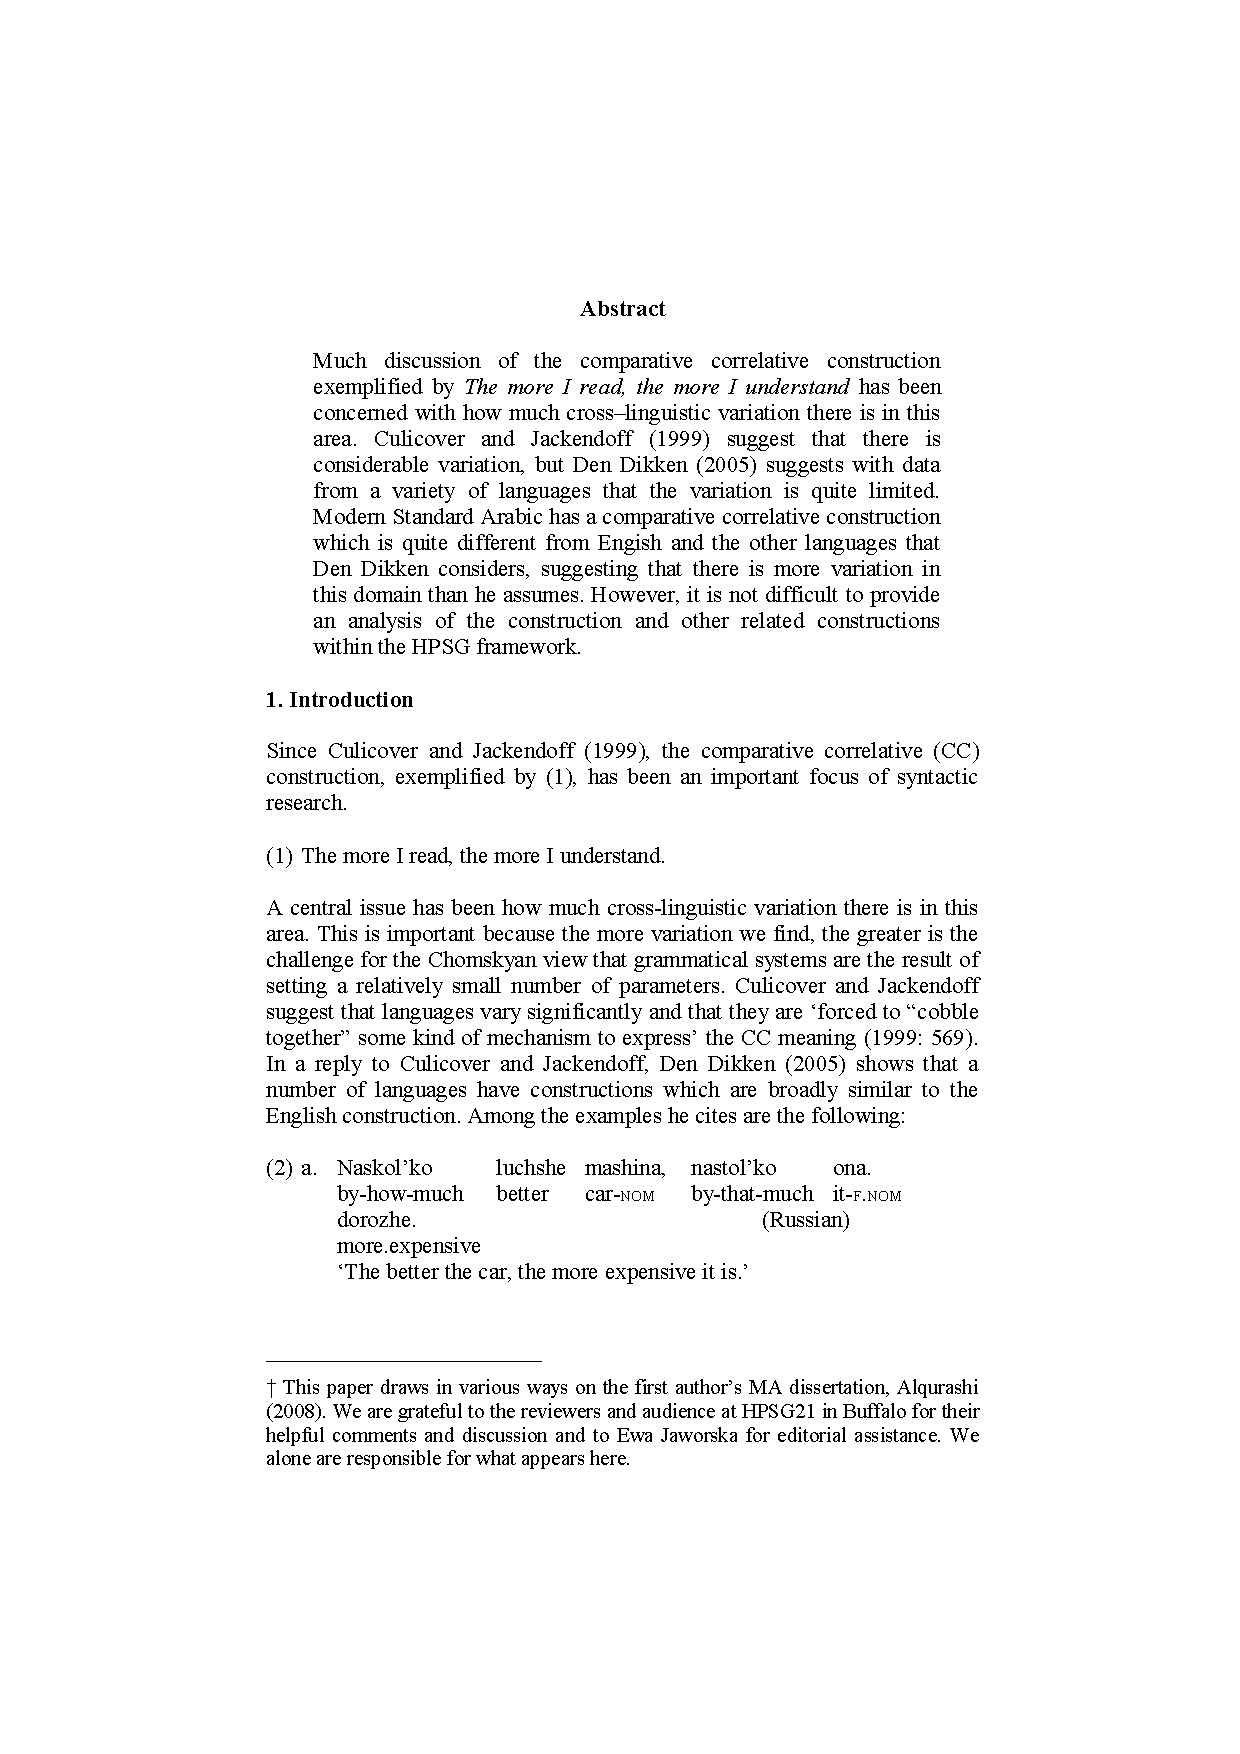
\includepdf[pages=-,pagecommand=\thispagestyle{plain}]{Includes/alqurashi-borsley.pdf}
        \setcounter{page}{27}
        \phantomsection
        \addcontentsline{toc}{section}{Doug Arnold, Robert D. Borsley: On the Analysis of English Exhaustive Conditionals}
\thispagestyle{empty}

\begin{center}
  {\huge\bfseries On the Analysis of English Exhaustive Conditionals\par}

  \bigskip

~\\
\begingroup
\setlength{\leftskip}{0pt plus 1fill}
\setlength{\rightskip}{0pt plus 1fill}
\setlength{\parindent}{0pt}
\setlength{\parfillskip}{0pt}
  \formatauthor{Doug Arnold}{\begin{tabular}{@{}c@{}}University of Essex\end{tabular}}
\formatauthor{Robert D. Borsley}{\begin{tabular}{@{}c@{}}University of Essex\end{tabular}}

\par\endgroup

  \vspace*{8ex}

  Proceedings of the 21st International Conference on\par Head-Driven Phrase Structure Grammar

  \bigskip

  University at Buffalo

  \medskip

  Stefan Müller (Editor)

  \medskip

  2014

  \medskip

  CSLI Publications

  \medskip

  pages 27--47

  \medskip

  \url{http://csli-publications.stanford.edu/HPSG/2014}
\end{center}
\vfill

\noindent



\vfill
\noindent
% APA Style
Arnold, Doug, \& Borsley, Robert D. 2014. On the Analysis of English Exhaustive Conditionals. In Müller, Stefan (Ed.), \emph{{Proceedings of the 21st International Conference on Head-Driven Phrase Structure Grammar, University at Buffalo}}, 27--47. Stanford,
CA: CSLI Publications. \hfill\href{http://creativecommons.org/licenses/by/4.0/}{\includegraphics[height=.75em]{Includes/ccby.eps}}

\newpage
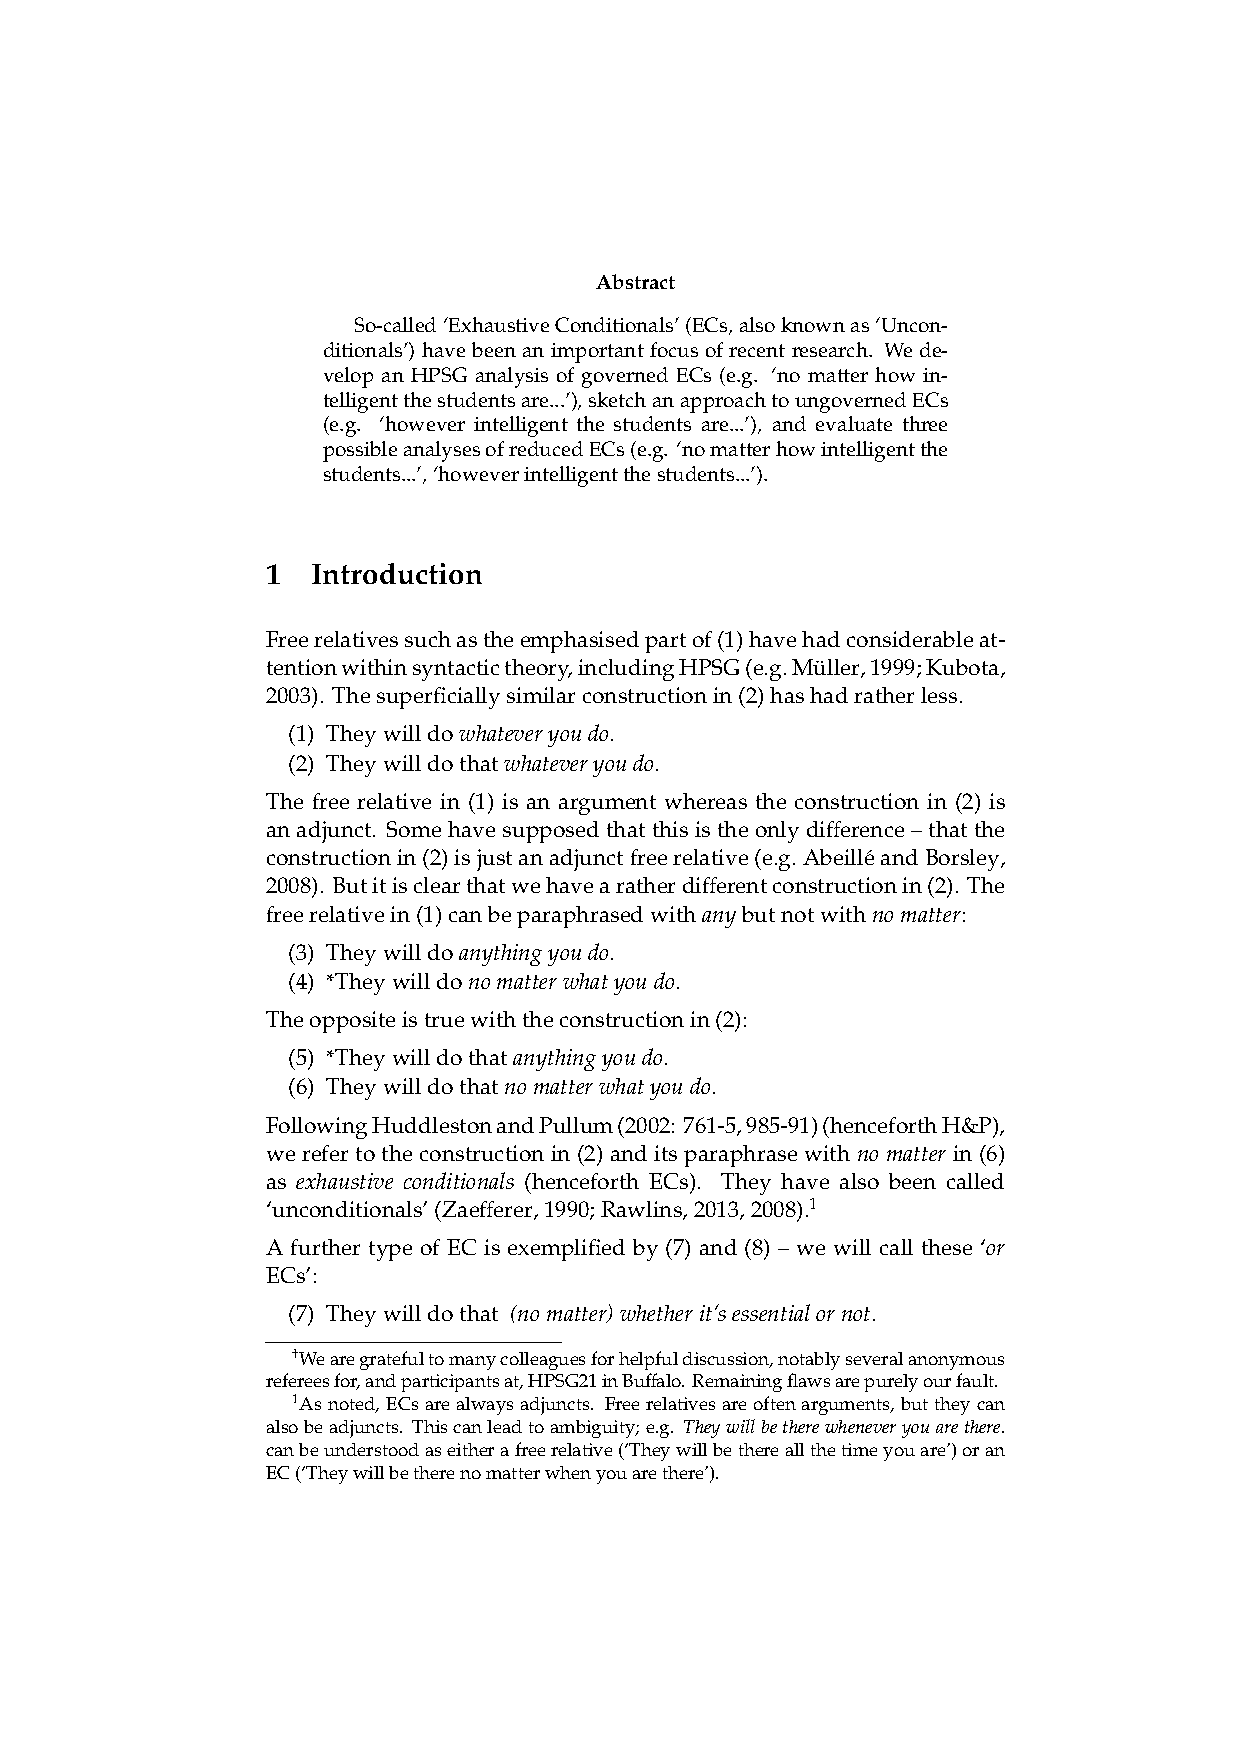
\includepdf[pages=-,pagecommand=\thispagestyle{plain}]{Includes/arnold-borsley.pdf}
        \setcounter{page}{48}
        \phantomsection
        \addcontentsline{toc}{section}{Philippa Cook: Between complex predicates and regular phrases: German collocational clusters}
\thispagestyle{empty}

\begin{center}
  {\huge\bfseries Between complex predicates and regular phrases: German collocational clusters\par}

  \bigskip

~\\
\begingroup
\setlength{\leftskip}{0pt plus 1fill}
\setlength{\rightskip}{0pt plus 1fill}
\setlength{\parindent}{0pt}
\setlength{\parfillskip}{0pt}
  \formatauthor{Philippa Cook}{\begin{tabular}{@{}c@{}}Freie Universität Berlin\end{tabular}}

\par\endgroup

  \vspace*{8ex}

  Proceedings of the 21st International Conference on\par Head-Driven Phrase Structure Grammar

  \bigskip

  University at Buffalo

  \medskip

  Stefan Müller (Editor)

  \medskip

  2014

  \medskip

  CSLI Publications

  \medskip

  pages 48--62

  \medskip

  \url{http://csli-publications.stanford.edu/HPSG/2014}
\end{center}
\vfill

\noindent



\vfill
\noindent
% APA Style
Cook, Philippa. 2014. Between complex predicates and regular phrases: German collocational clusters. In Müller, Stefan (Ed.), \emph{{Proceedings of the 21st International Conference on Head-Driven Phrase Structure Grammar, University at Buffalo}}, 48--62. Stanford,
CA: CSLI Publications. \hfill\href{http://creativecommons.org/licenses/by/4.0/}{\includegraphics[height=.75em]{Includes/ccby.eps}}

\newpage
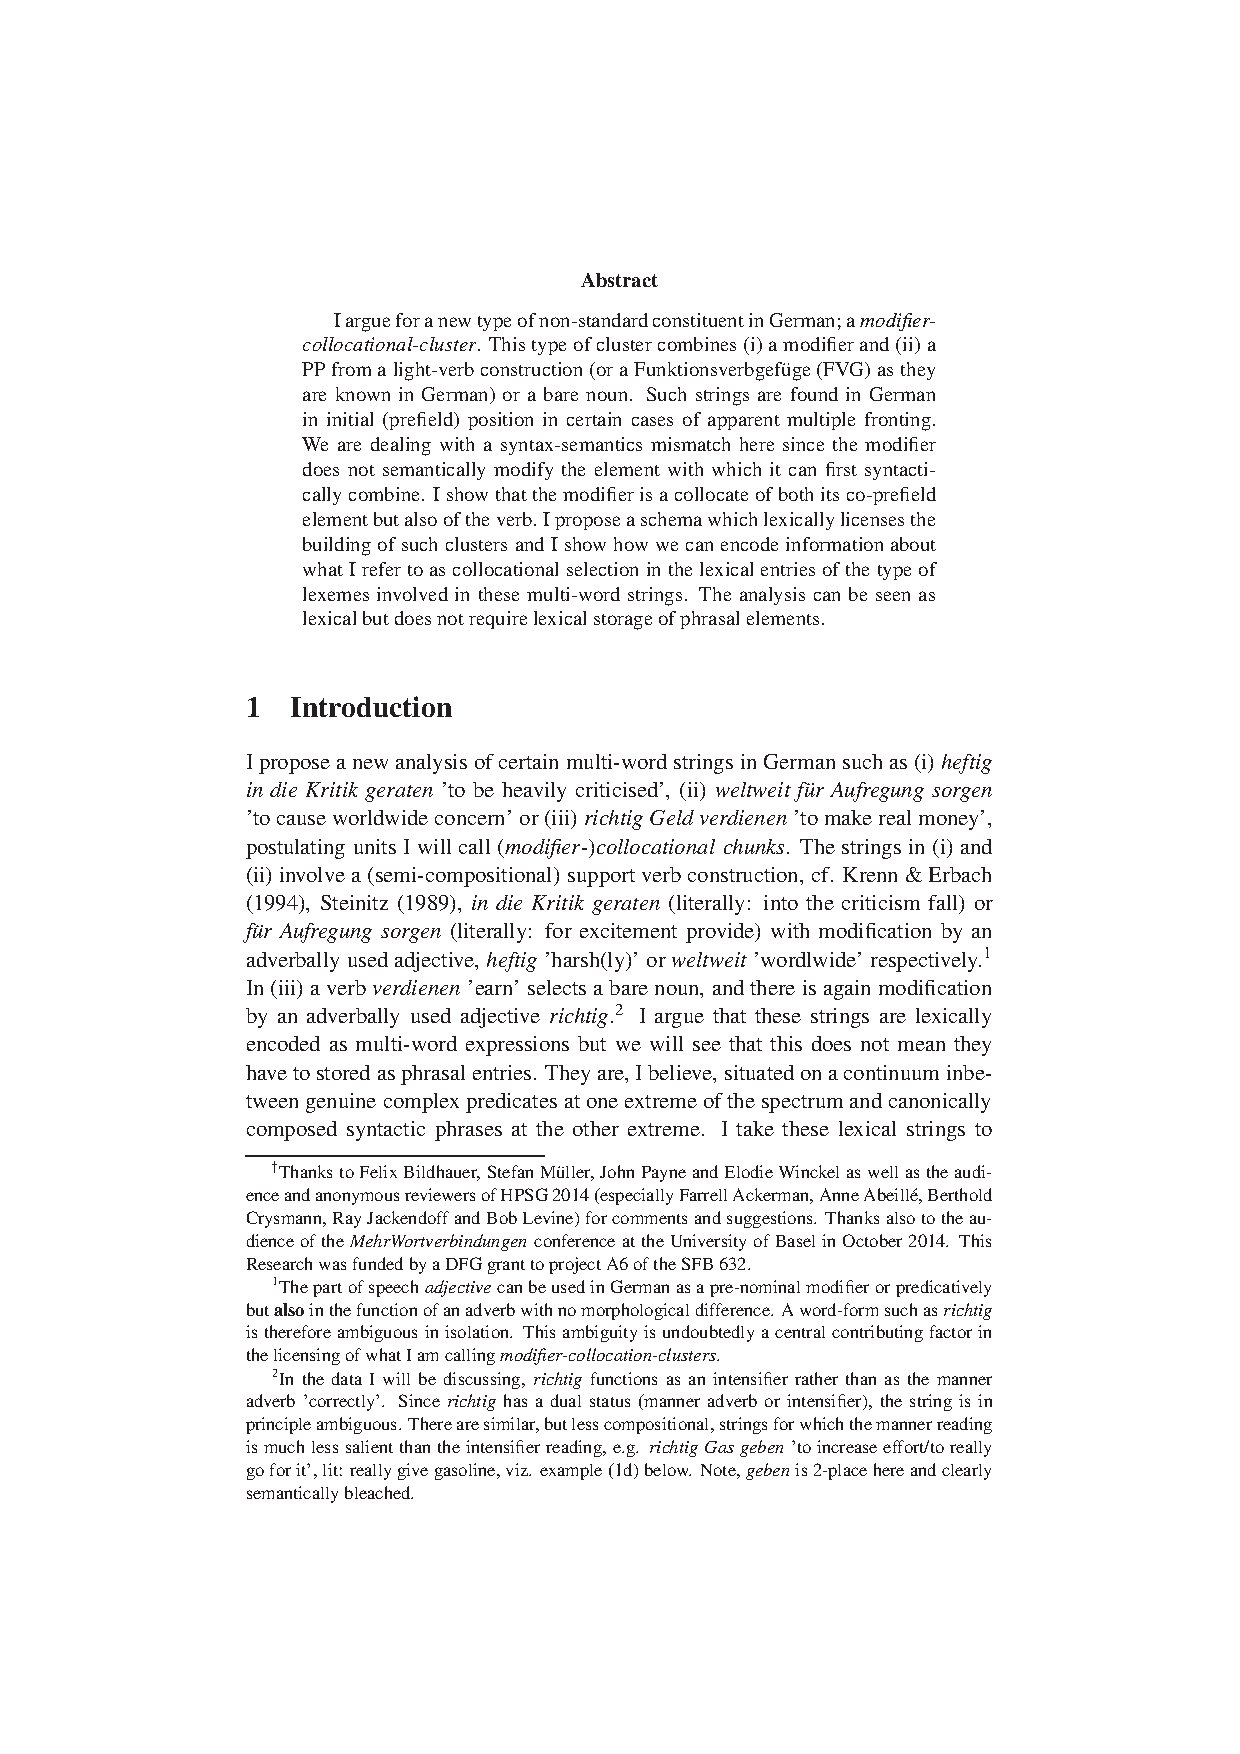
\includepdf[pages=-,pagecommand=\thispagestyle{plain}]{Includes/cook.pdf}
        \setcounter{page}{63}
        \phantomsection
        \addcontentsline{toc}{section}{Berthold Crysmann, Chris H. Reintges: The Polyfunctionality of {Coptic} {Egyptian} Relative Complementisers}
\thispagestyle{empty}

\begin{center}
  {\huge\bfseries The Polyfunctionality of {Coptic} {Egyptian} Relative Complementisers\par}

  \bigskip

~\\
\begingroup
\setlength{\leftskip}{0pt plus 1fill}
\setlength{\rightskip}{0pt plus 1fill}
\setlength{\parindent}{0pt}
\setlength{\parfillskip}{0pt}
  \formatauthor{Berthold Crysmann}{\begin{tabular}{@{}c@{}}CNRS, Laboratoire de linguistique formelle\end{tabular}}
\formatauthor{Chris H. Reintges}{\begin{tabular}{@{}c@{}}CNRS, Laboratoire de linguistique formelle\end{tabular}}

\par\endgroup

  \vspace*{8ex}

  Proceedings of the 21st International Conference on\par Head-Driven Phrase Structure Grammar

  \bigskip

  University at Buffalo

  \medskip

  Stefan Müller (Editor)

  \medskip

  2014

  \medskip

  CSLI Publications

  \medskip

  pages 63--82

  \medskip

  \url{http://csli-publications.stanford.edu/HPSG/2014}
\end{center}
\vfill

\noindent



\vfill
\noindent
% APA Style
Crysmann, Berthold, \& Reintges, Chris H. 2014. The Polyfunctionality of {Coptic} {Egyptian} Relative Complementisers. In Müller, Stefan (Ed.), \emph{{Proceedings of the 21st International Conference on Head-Driven Phrase Structure Grammar, University at Buffalo}}, 63--82. Stanford,
CA: CSLI Publications. \hfill\href{http://creativecommons.org/licenses/by/4.0/}{\includegraphics[height=.75em]{Includes/ccby.eps}}

\newpage
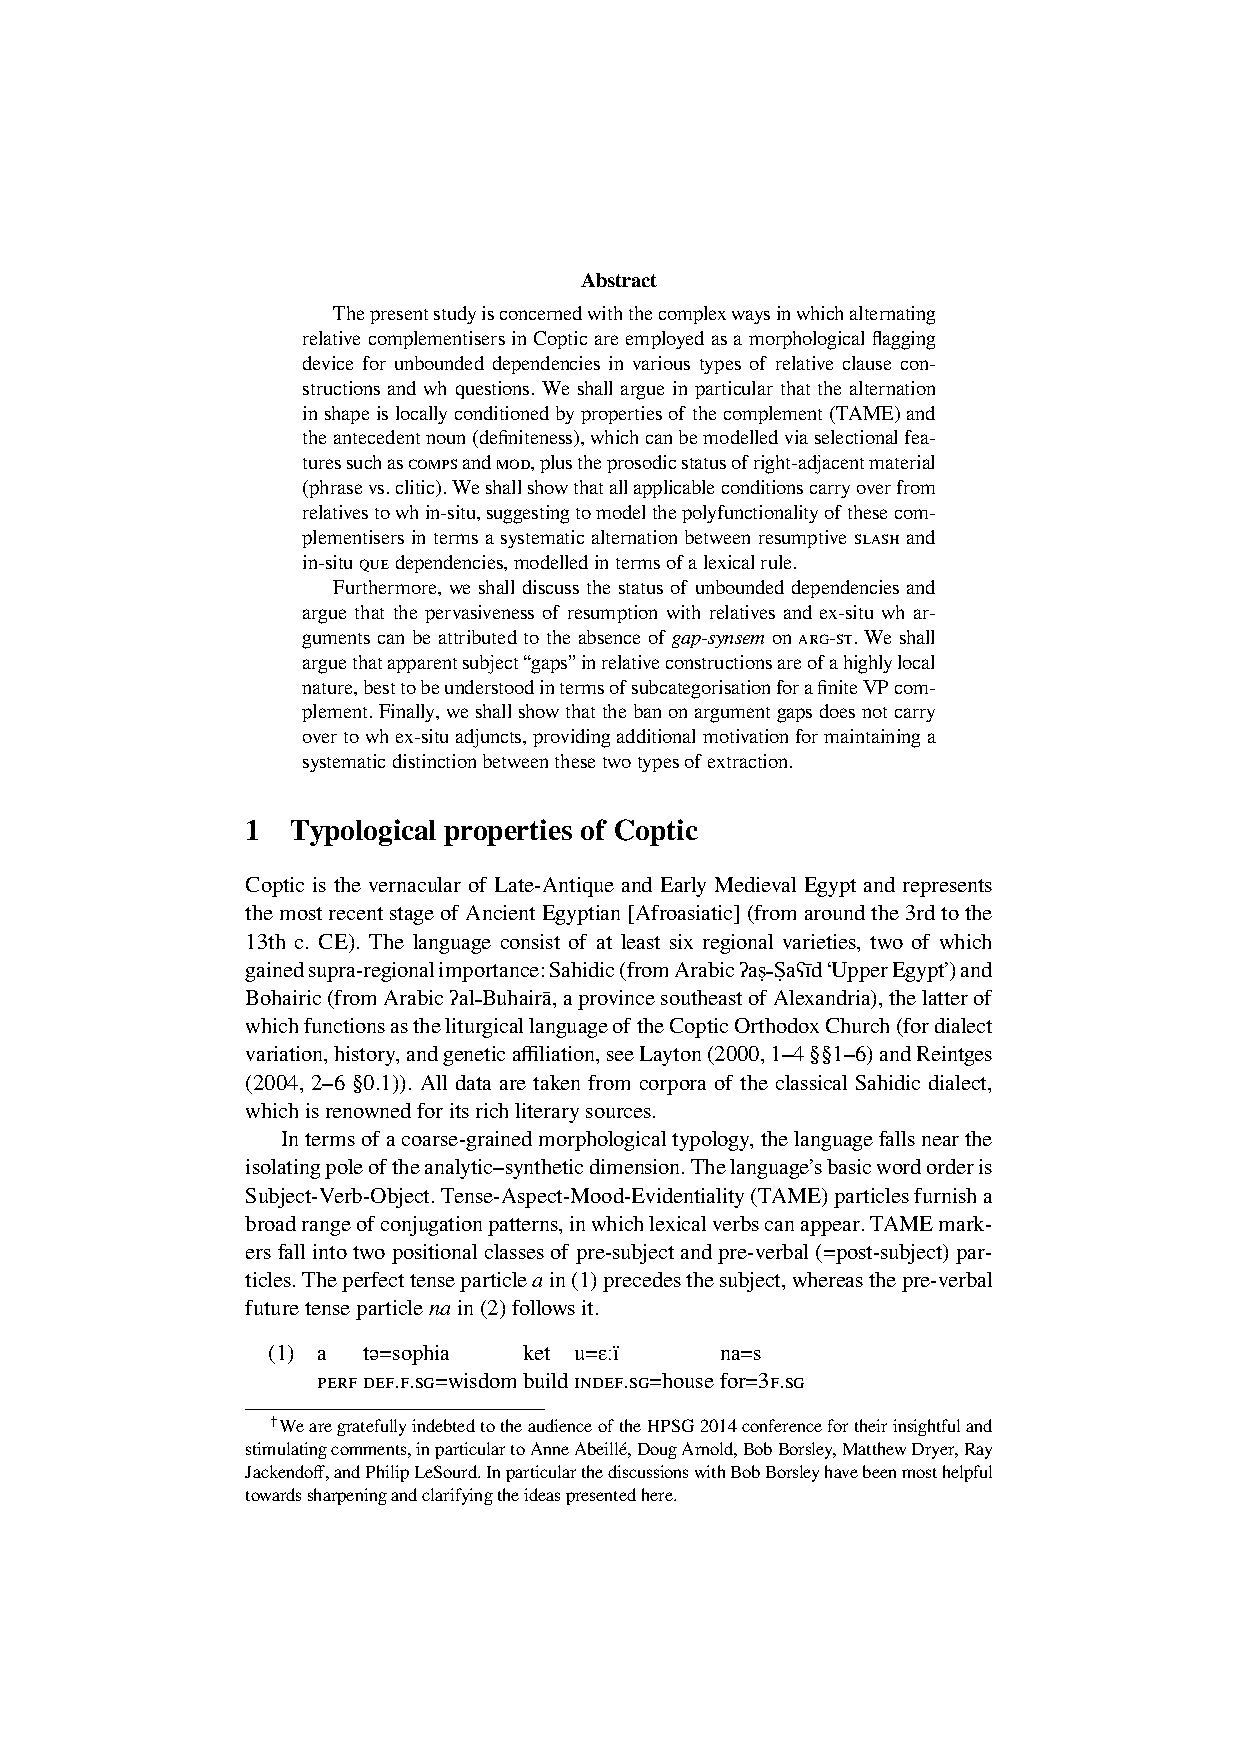
\includepdf[pages=-,pagecommand=\thispagestyle{plain}]{Includes/crysmann-reintges.pdf}
        \setcounter{page}{83}
        \phantomsection
        \addcontentsline{toc}{section}{Petter Haugereid: VP idioms in Norwegian:\\ A subconstructional approach}
\thispagestyle{empty}

\begin{center}
  {\huge\bfseries VP idioms in Norwegian:\par A subconstructional approach\par}

  \bigskip

~\\
\begingroup
\setlength{\leftskip}{0pt plus 1fill}
\setlength{\rightskip}{0pt plus 1fill}
\setlength{\parindent}{0pt}
\setlength{\parfillskip}{0pt}
  \formatauthor{Petter Haugereid}{\begin{tabular}{@{}c@{}}Bergen University College\end{tabular}}

\par\endgroup

  \vspace*{8ex}

  Proceedings of the 21st International Conference on\par Head-Driven Phrase Structure Grammar

  \bigskip

  University at Buffalo

  \medskip

  Stefan Müller (Editor)

  \medskip

  2014

  \medskip

  CSLI Publications

  \medskip

  pages 83--102

  \medskip

  \url{http://csli-publications.stanford.edu/HPSG/2014}
\end{center}
\vfill

\noindent



\vfill
\noindent
% APA Style
Haugereid, Petter. 2014. VP idioms in Norwegian:  A subconstructional approach. In Müller, Stefan (Ed.), \emph{{Proceedings of the 21st International Conference on Head-Driven Phrase Structure Grammar, University at Buffalo}}, 83--102. Stanford,
CA: CSLI Publications. \hfill\href{http://creativecommons.org/licenses/by/4.0/}{\includegraphics[height=.75em]{Includes/ccby.eps}}

\newpage
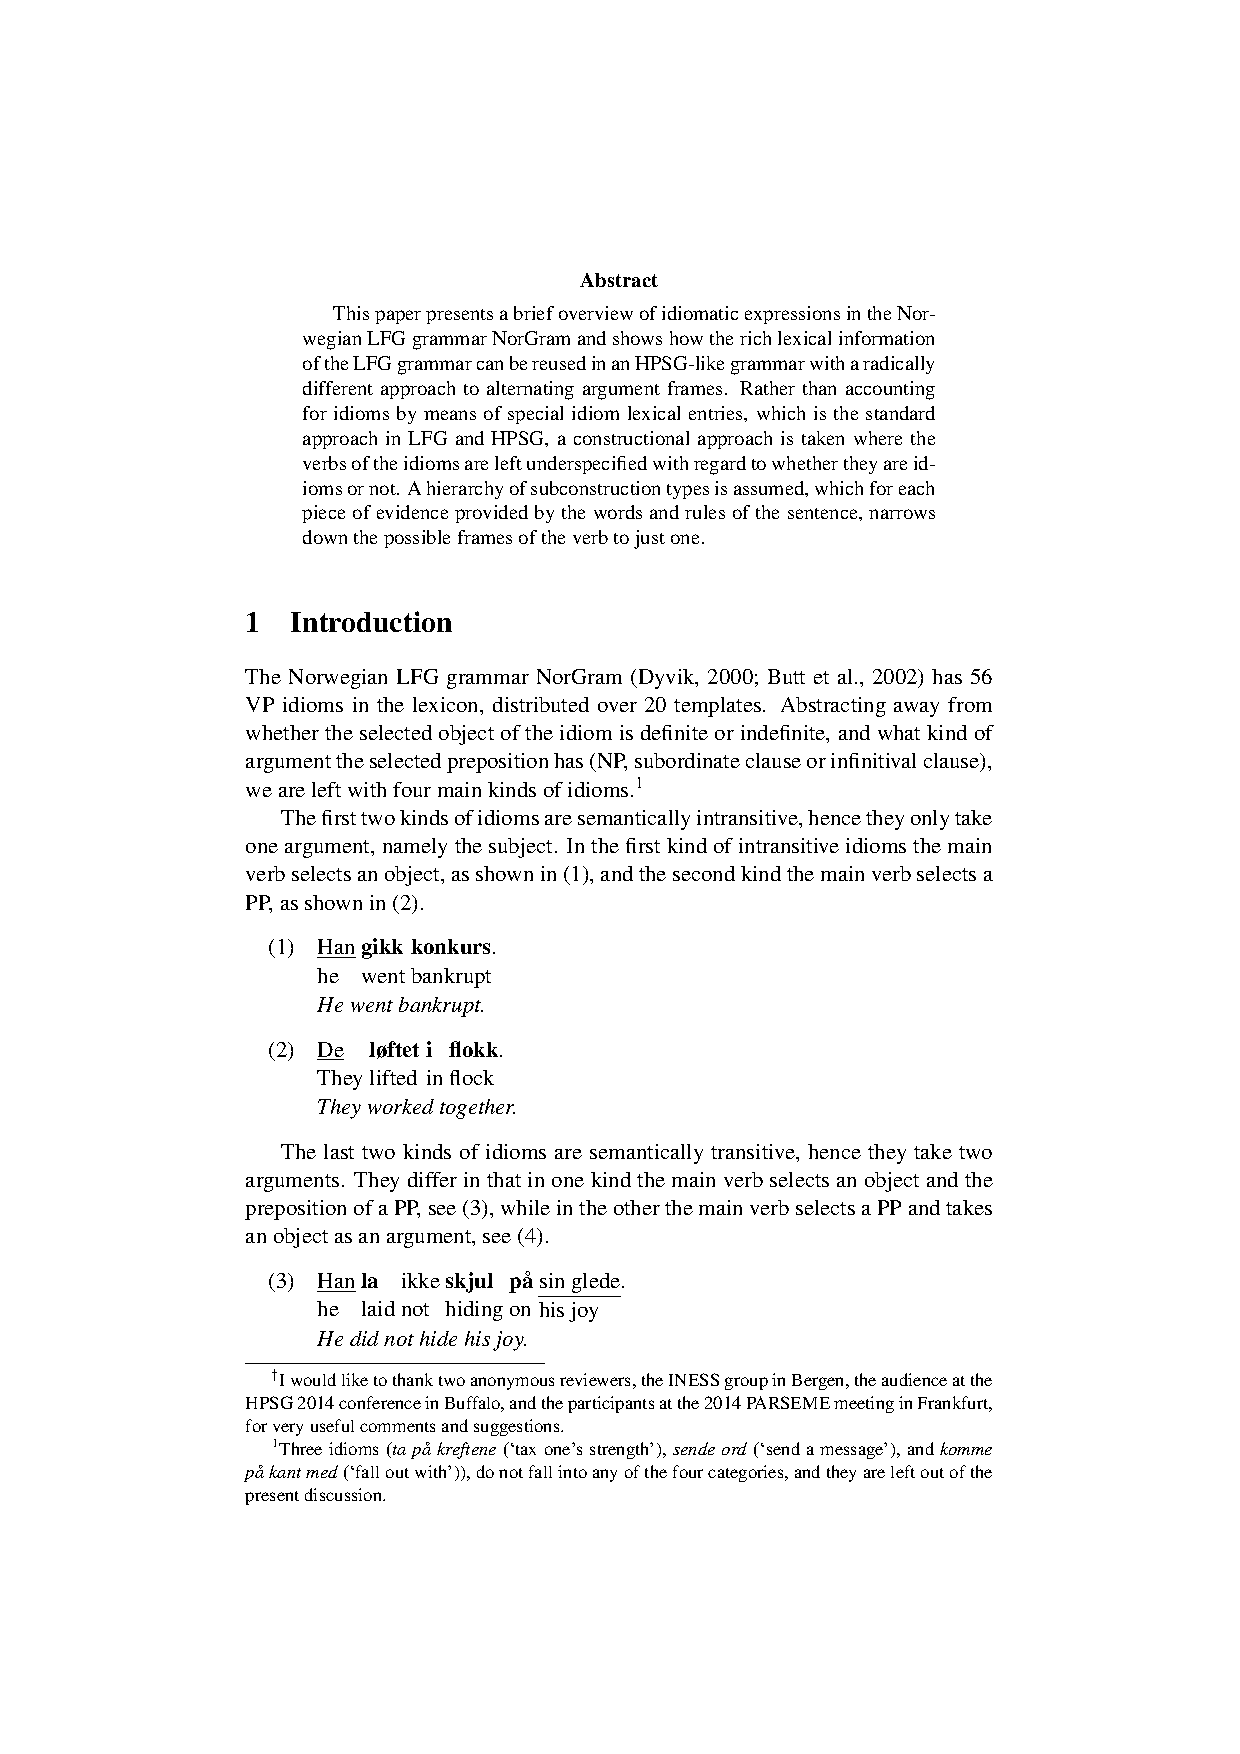
\includepdf[pages=-,pagecommand=\thispagestyle{plain}]{Includes/haugereid.pdf}
        \setcounter{page}{103}
        \phantomsection
        \addcontentsline{toc}{section}{David Inman, Ruth Morrison: Negation in Nanti: Syntactic Evidence for Head and Dependent Negators}
\thispagestyle{empty}

\begin{center}
  {\huge\bfseries Negation in Nanti: Syntactic Evidence for Head and Dependent Negators\par}

  \bigskip

~\\
\begingroup
\setlength{\leftskip}{0pt plus 1fill}
\setlength{\rightskip}{0pt plus 1fill}
\setlength{\parindent}{0pt}
\setlength{\parfillskip}{0pt}
  \formatauthor{David Inman}{\begin{tabular}{@{}c@{}}University of Washington\end{tabular}}
\formatauthor{Ruth Morrison}{\begin{tabular}{@{}c@{}}University of Washington\end{tabular}}

\par\endgroup

  \vspace*{8ex}

  Proceedings of the 21st International Conference on\par Head-Driven Phrase Structure Grammar

  \bigskip

  University at Buffalo

  \medskip

  Stefan Müller (Editor)

  \medskip

  2014

  \medskip

  CSLI Publications

  \medskip

  pages 103--113

  \medskip

  \url{http://csli-publications.stanford.edu/HPSG/2014}
\end{center}
\vfill

\noindent



\vfill
\noindent
% APA Style
Inman, David, \& Morrison, Ruth. 2014. Negation in Nanti: Syntactic Evidence for Head and Dependent Negators. In Müller, Stefan (Ed.), \emph{{Proceedings of the 21st International Conference on Head-Driven Phrase Structure Grammar, University at Buffalo}}, 103--113. Stanford,
CA: CSLI Publications. \hfill\href{http://creativecommons.org/licenses/by/4.0/}{\includegraphics[height=.75em]{Includes/ccby.eps}}

\newpage
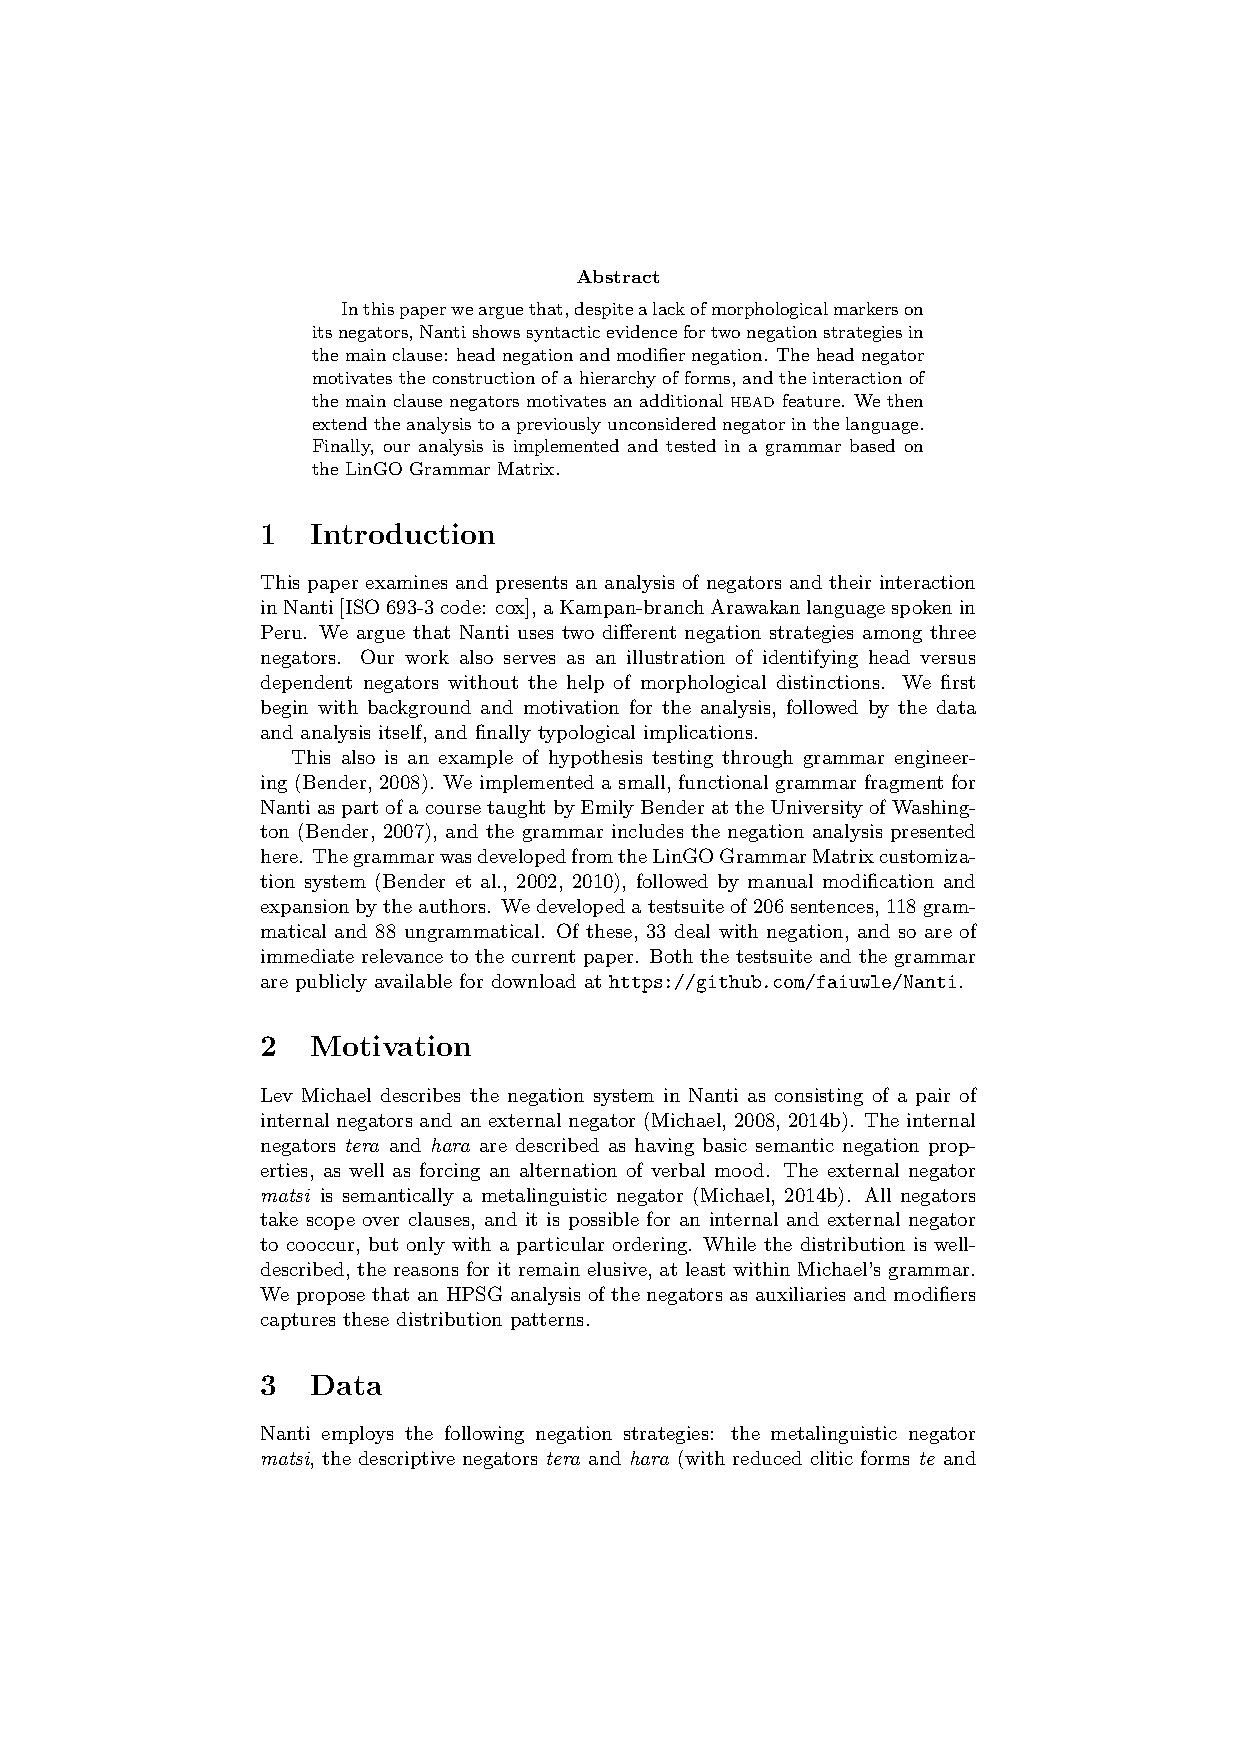
\includepdf[pages=-,pagecommand=\thispagestyle{plain}]{Includes/inman-morrison.pdf}
        \setcounter{page}{114}
        \phantomsection
        \addcontentsline{toc}{section}{Jean-Pierre Koenig, Karin Michelson: Deconstructing SYNtax}
\thispagestyle{empty}

\begin{center}
  {\huge\bfseries Deconstructing SYNtax\par}

  \bigskip

~\\
\begingroup
\setlength{\leftskip}{0pt plus 1fill}
\setlength{\rightskip}{0pt plus 1fill}
\setlength{\parindent}{0pt}
\setlength{\parfillskip}{0pt}
  \formatauthor{Jean-Pierre Koenig}{\begin{tabular}{@{}c@{}}University at Buffalo\end{tabular}}
\formatauthor{Karin Michelson}{\begin{tabular}{@{}c@{}}University at Buffalo\end{tabular}}

\par\endgroup

  \vspace*{8ex}

  Proceedings of the 21st International Conference on\par Head-Driven Phrase Structure Grammar

  \bigskip

  University at Buffalo

  \medskip

  Stefan Müller (Editor)

  \medskip

  2014

  \medskip

  CSLI Publications

  \medskip

  pages 114--134

  \medskip

  \url{http://csli-publications.stanford.edu/HPSG/2014}
\end{center}
\vfill

\noindent



\vfill
\noindent
% APA Style
Koenig, Jean-Pierre, \& Michelson, Karin. 2014. Deconstructing SYNtax. In Müller, Stefan (Ed.), \emph{{Proceedings of the 21st International Conference on Head-Driven Phrase Structure Grammar, University at Buffalo}}, 114--134. Stanford,
CA: CSLI Publications. \hfill\href{http://creativecommons.org/licenses/by/4.0/}{\includegraphics[height=.75em]{Includes/ccby.eps}}

\newpage
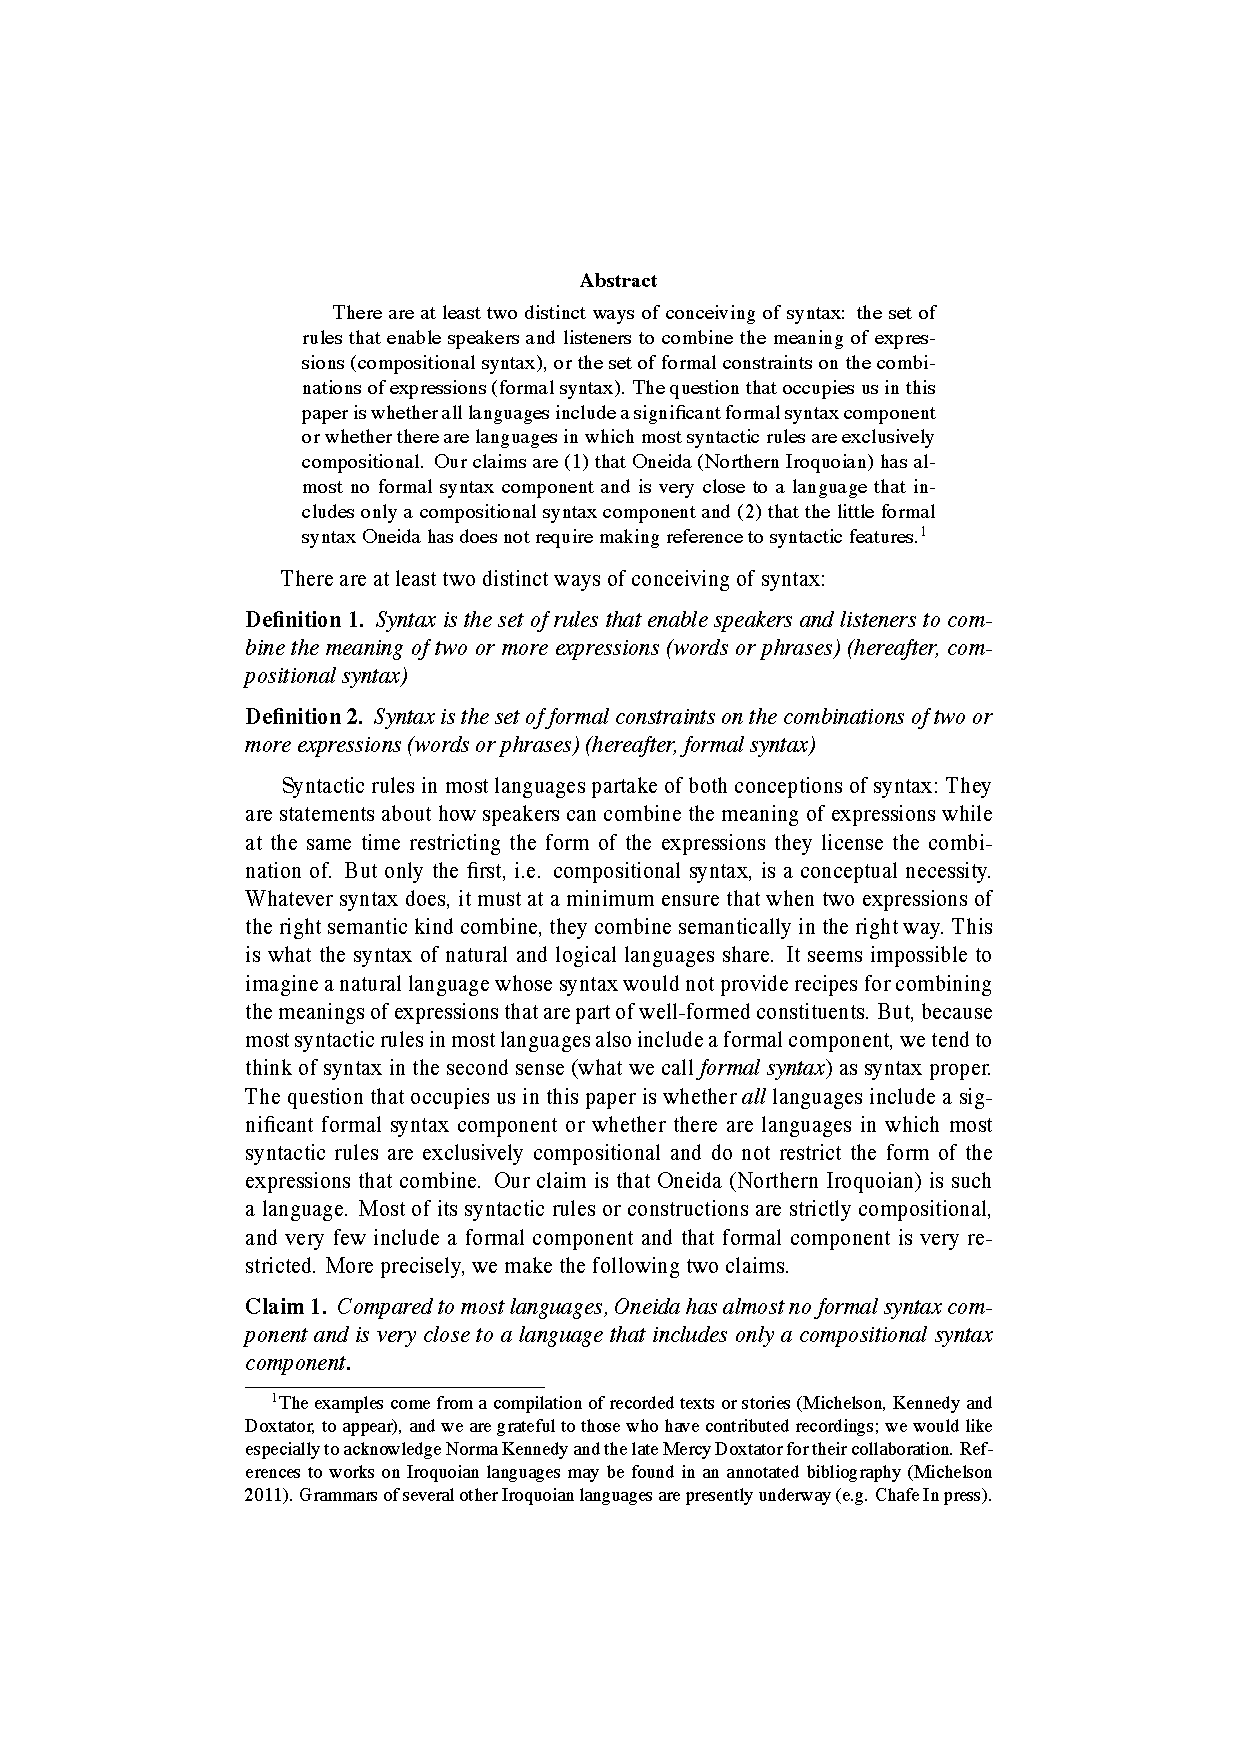
\includepdf[pages=-,pagecommand=\thispagestyle{plain}]{Includes/koenig-michelson.pdf}
        \setcounter{page}{135}
        \phantomsection
        \addcontentsline{toc}{section}{Juwon Lee: Two Types of Serial Verb Constructions in Korean: Subject-Sharing and Index-Sharing}
\thispagestyle{empty}

\begin{center}
  {\huge\bfseries Two Types of Serial Verb Constructions in Korean: Subject-Sharing and Index-Sharing\par}

  \bigskip

~\\
\begingroup
\setlength{\leftskip}{0pt plus 1fill}
\setlength{\rightskip}{0pt plus 1fill}
\setlength{\parindent}{0pt}
\setlength{\parfillskip}{0pt}
  \formatauthor{Juwon Lee}{\begin{tabular}{@{}c@{}}The University of Texas at Austin\end{tabular}}

\par\endgroup

  \vspace*{8ex}

  Proceedings of the 21st International Conference on\par Head-Driven Phrase Structure Grammar

  \bigskip

  University at Buffalo

  \medskip

  Stefan Müller (Editor)

  \medskip

  2014

  \medskip

  CSLI Publications

  \medskip

  pages 135--155

  \medskip

  \url{http://csli-publications.stanford.edu/HPSG/2014}
\end{center}
\vfill

\noindent



\vfill
\noindent
% APA Style
Lee, Juwon. 2014. Two Types of Serial Verb Constructions in Korean: Subject-Sharing and Index-Sharing. In Müller, Stefan (Ed.), \emph{{Proceedings of the 21st International Conference on Head-Driven Phrase Structure Grammar, University at Buffalo}}, 135--155. Stanford,
CA: CSLI Publications. \hfill\href{http://creativecommons.org/licenses/by/4.0/}{\includegraphics[height=.75em]{Includes/ccby.eps}}

\newpage
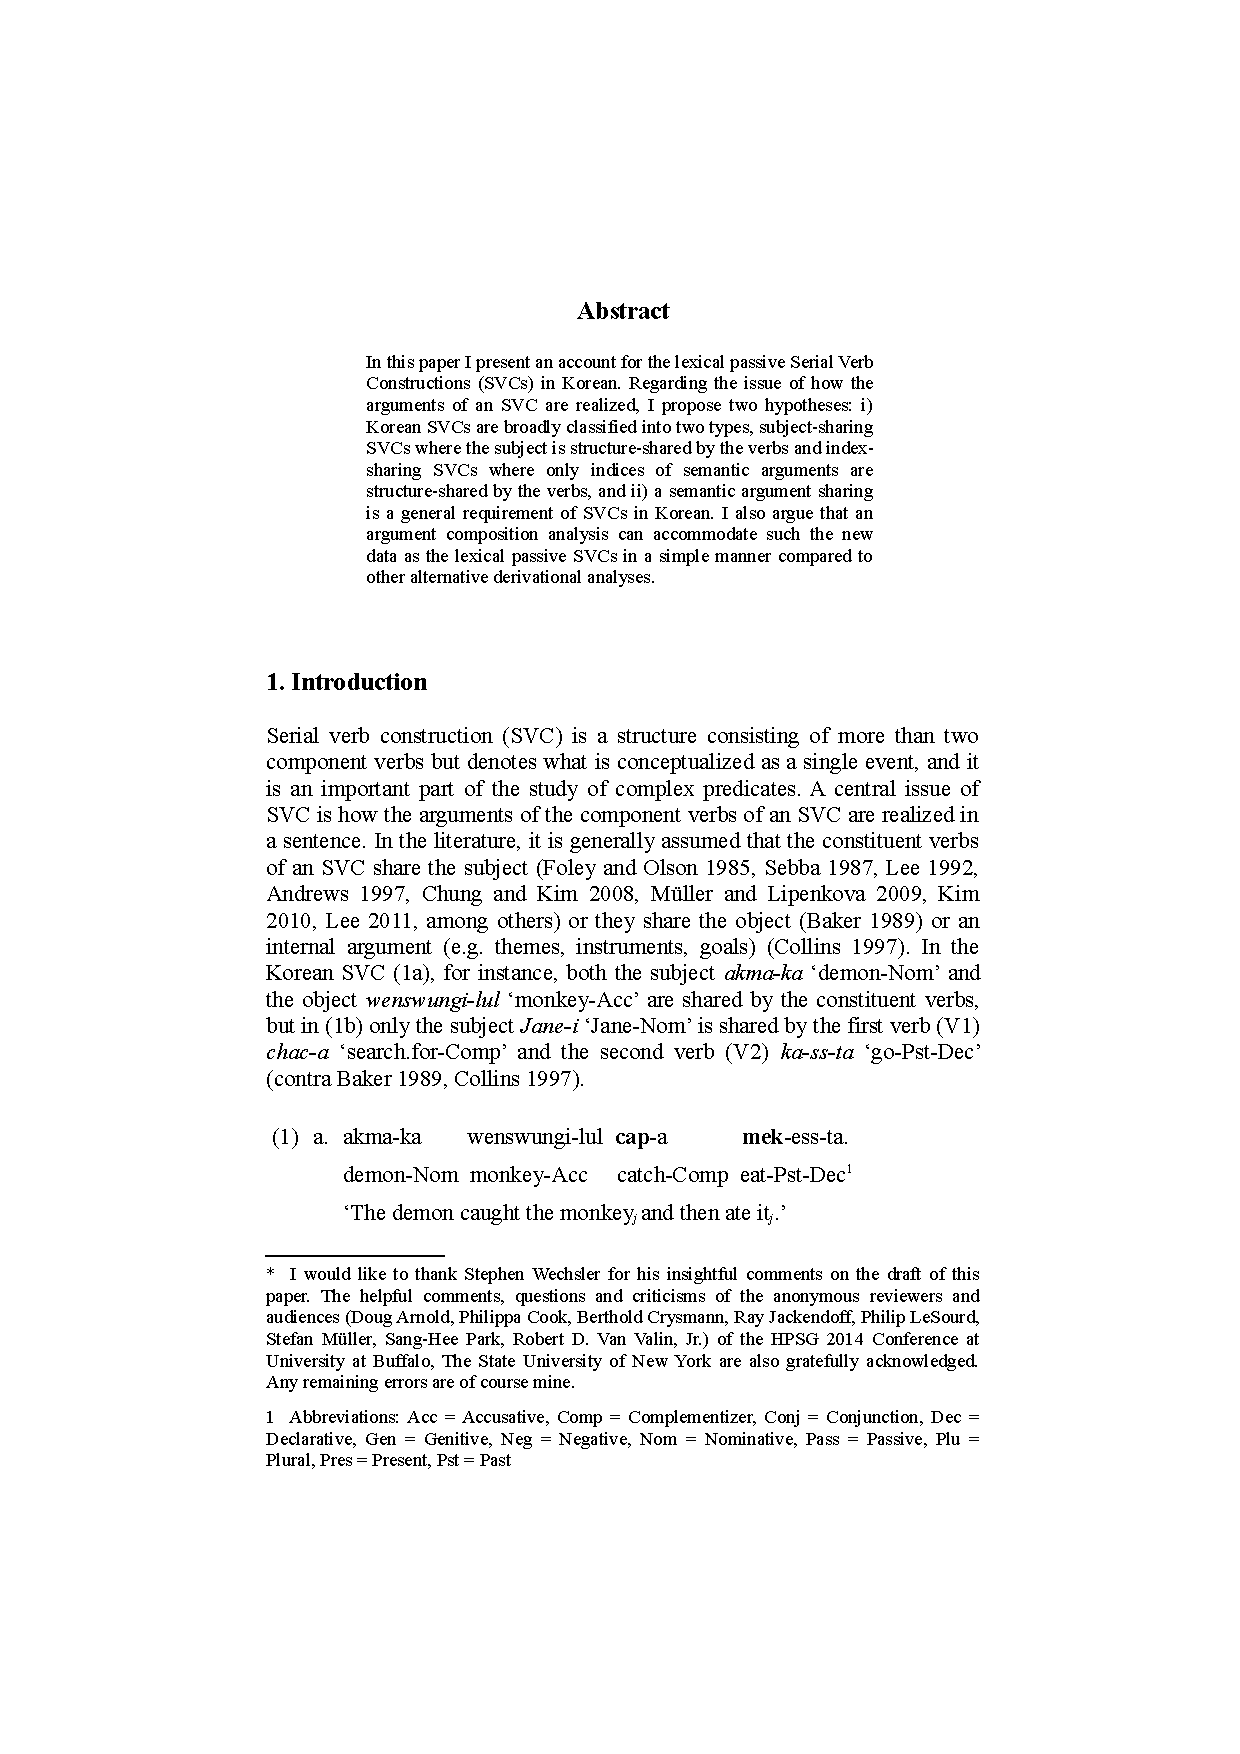
\includepdf[pages=-,pagecommand=\thispagestyle{plain}]{Includes/lee.pdf}
        \setcounter{page}{156}
        \phantomsection
        \addcontentsline{toc}{section}{Frank Van Eynde, Liesbeth Augustinus: Complement Raising, Extraction and Adpostion Stranding in Dutch}
\thispagestyle{empty}

\begin{center}
  {\huge\bfseries Complement Raising, Extraction and Adpostion Stranding in Dutch\par}

  \bigskip

~\\
\begingroup
\setlength{\leftskip}{0pt plus 1fill}
\setlength{\rightskip}{0pt plus 1fill}
\setlength{\parindent}{0pt}
\setlength{\parfillskip}{0pt}
  \formatauthor{Frank Van Eynde}{\begin{tabular}{@{}c@{}}University of Leuven\end{tabular}}
\formatauthor{Liesbeth Augustinus}{\begin{tabular}{@{}c@{}}University of Leuven\end{tabular}}

\par\endgroup

  \vspace*{8ex}

  Proceedings of the 21st International Conference on\par Head-Driven Phrase Structure Grammar

  \bigskip

  University at Buffalo

  \medskip

  Stefan Müller (Editor)

  \medskip

  2014

  \medskip

  CSLI Publications

  \medskip

  pages 156--175

  \medskip

  \url{http://csli-publications.stanford.edu/HPSG/2014}
\end{center}
\vfill

\noindent



\vfill
\noindent
% APA Style
Van Eynde, Frank, \& Augustinus, Liesbeth. 2014. Complement Raising, Extraction and Adpostion Stranding in Dutch. In Müller, Stefan (Ed.), \emph{{Proceedings of the 21st International Conference on Head-Driven Phrase Structure Grammar, University at Buffalo}}, 156--175. Stanford,
CA: CSLI Publications. \hfill\href{http://creativecommons.org/licenses/by/4.0/}{\includegraphics[height=.75em]{Includes/ccby.eps}}

\newpage
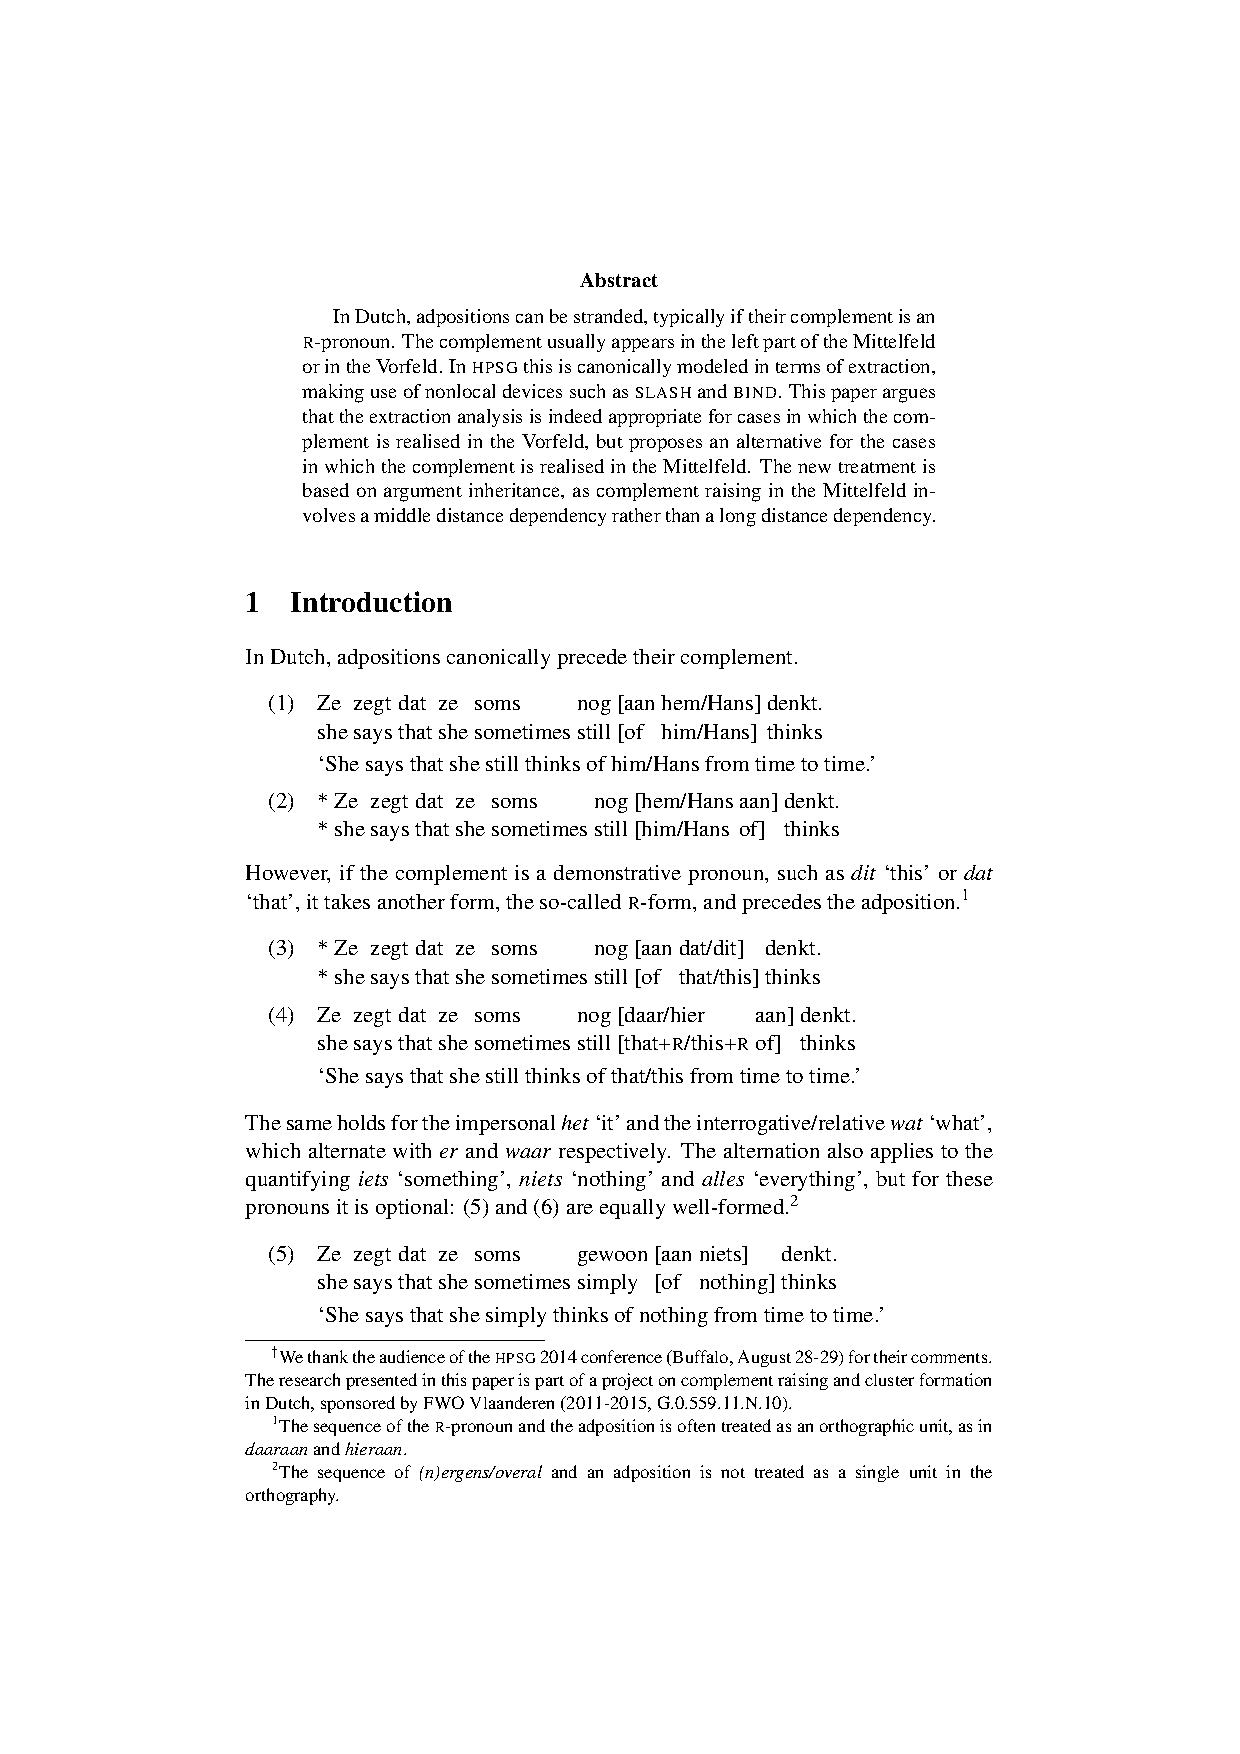
\includepdf[pages=-,pagecommand=\thispagestyle{plain}]{Includes/vaneynde-augustinus.pdf}
        \setcounter{page}{176}
        \phantomsection
        \addcontentsline{toc}{section}{Olga Zamaraeva, Emily M. Bender: Focus Case Outside of Austronesian:\\ An Analysis of Kolyma Yukaghir}
\thispagestyle{empty}

\begin{center}
  {\huge\bfseries Focus Case Outside of Austronesian:\par An Analysis of Kolyma Yukaghir\par}

  \bigskip

~\\
\begingroup
\setlength{\leftskip}{0pt plus 1fill}
\setlength{\rightskip}{0pt plus 1fill}
\setlength{\parindent}{0pt}
\setlength{\parfillskip}{0pt}
  \formatauthor{Olga Zamaraeva}{\begin{tabular}{@{}c@{}}University of Washington\end{tabular}}
\formatauthor{Emily M. Bender}{\begin{tabular}{@{}c@{}}University of Washington\end{tabular}}

\par\endgroup

  \vspace*{8ex}

  Proceedings of the 21st International Conference on\par Head-Driven Phrase Structure Grammar

  \bigskip

  University at Buffalo

  \medskip

  Stefan Müller (Editor)

  \medskip

  2014

  \medskip

  CSLI Publications

  \medskip

  pages 176--196

  \medskip

  \url{http://csli-publications.stanford.edu/HPSG/2014}
\end{center}
\vfill

\noindent



\vfill
\noindent
% APA Style
Zamaraeva, Olga, \& Bender, Emily M. 2014. Focus Case Outside of Austronesian:  An Analysis of Kolyma Yukaghir. In Müller, Stefan (Ed.), \emph{{Proceedings of the 21st International Conference on Head-Driven Phrase Structure Grammar, University at Buffalo}}, 176--196. Stanford,
CA: CSLI Publications. \hfill\href{http://creativecommons.org/licenses/by/4.0/}{\includegraphics[height=.75em]{Includes/ccby.eps}}

\newpage
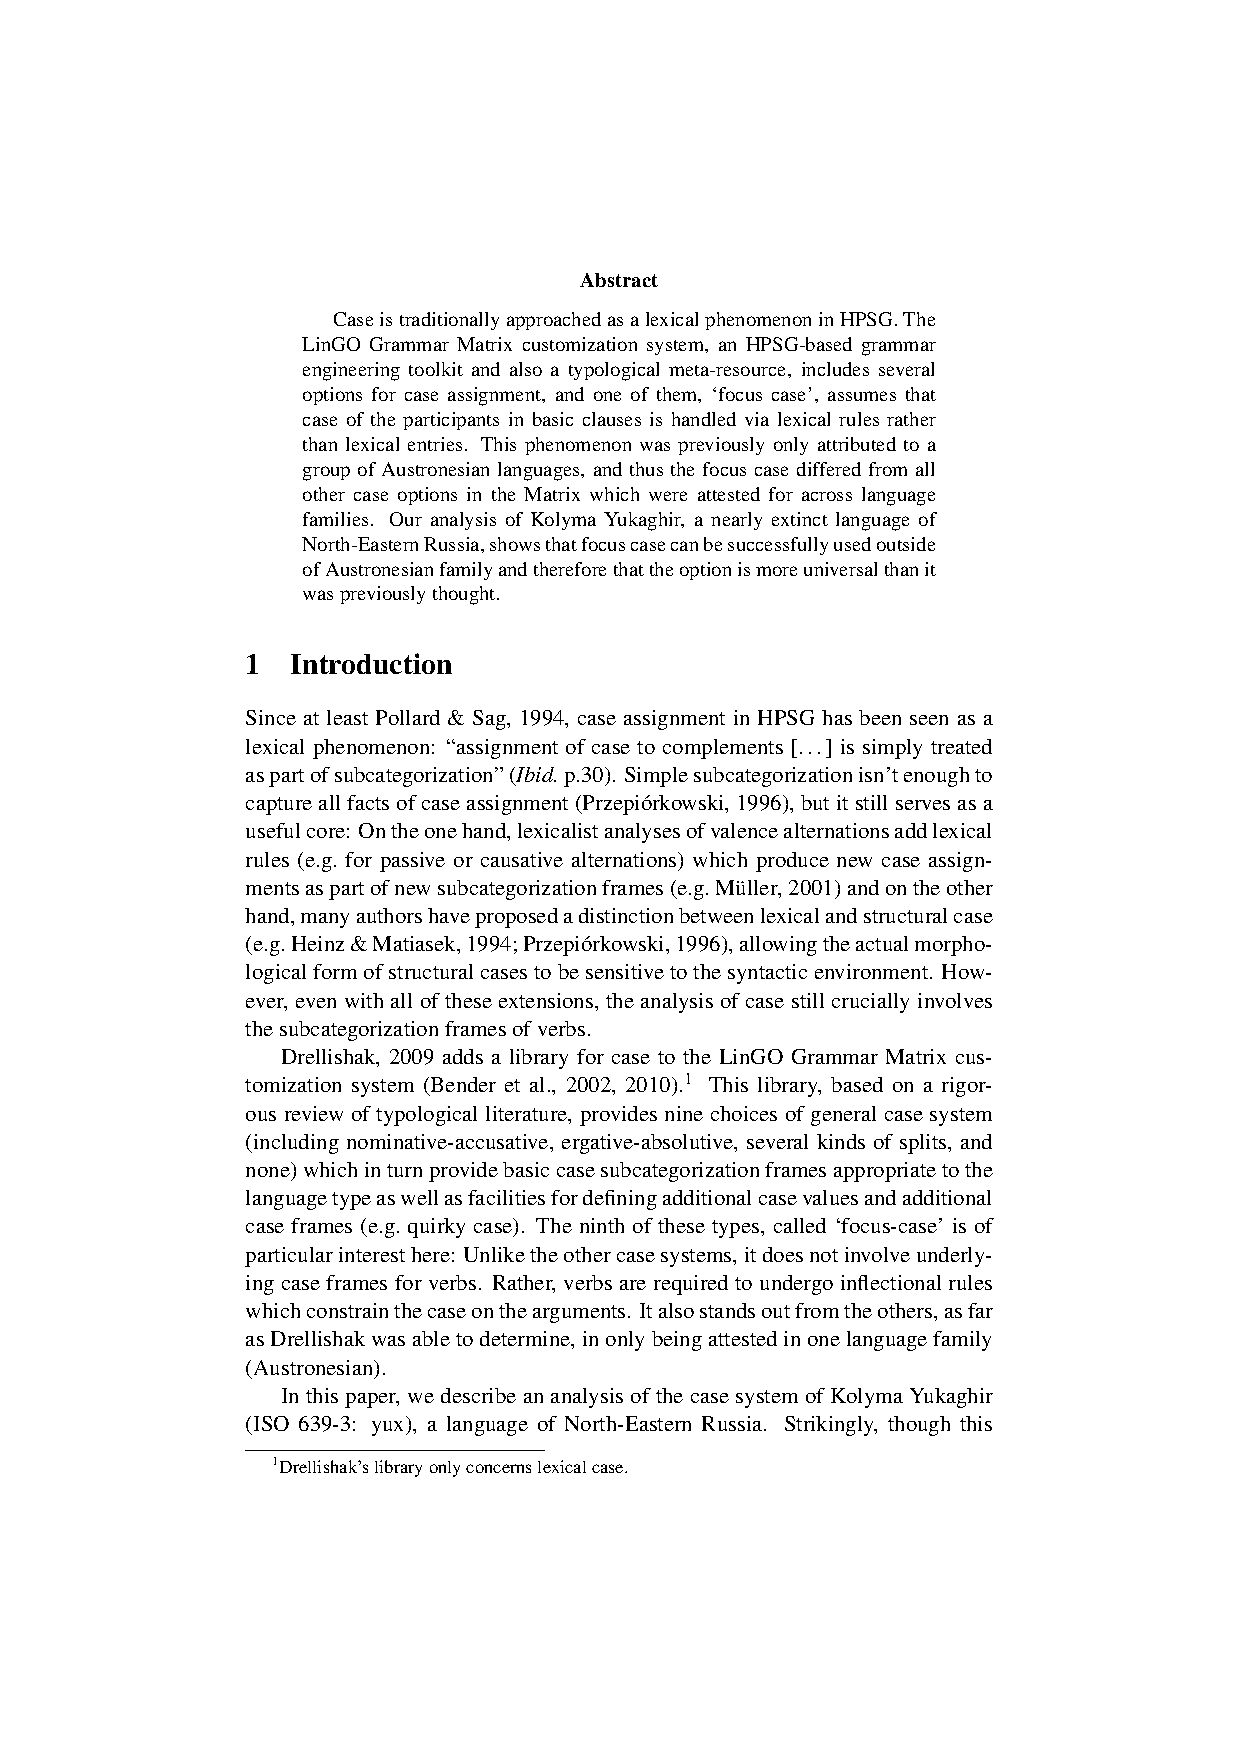
\includepdf[pages=-,pagecommand=\thispagestyle{plain}]{Includes/zamaraeva-bender.pdf}
\part{Contributions to the Workshop}
\thispagestyle{empty}
\newpage
        \setcounter{page}{198}
        \phantomsection
        \addcontentsline{toc}{section}{George Aaron Broadwell: Language description and the lexicon: Verbs of wearing in two Oaxacan languages}
\thispagestyle{empty}

\begin{center}
  {\huge\bfseries Language description and the lexicon: Verbs of wearing in two Oaxacan languages\par}

  \bigskip

~\\
\begingroup
\setlength{\leftskip}{0pt plus 1fill}
\setlength{\rightskip}{0pt plus 1fill}
\setlength{\parindent}{0pt}
\setlength{\parfillskip}{0pt}
  \formatauthor{George Aaron Broadwell}{\begin{tabular}{@{}c@{}}University at Albany, State University of New York\end{tabular}}

\par\endgroup

  \vspace*{8ex}

  Proceedings of the 21st International Conference on\par Head-Driven Phrase Structure Grammar

  \bigskip

  University at Buffalo

  \medskip

  Stefan Müller (Editor)

  \medskip

  2014

  \medskip

  CSLI Publications

  \medskip

  pages 198--216

  \medskip

  \url{http://csli-publications.stanford.edu/HPSG/2014}
\end{center}
\vfill

\noindent



\vfill
\noindent
% APA Style
Broadwell, George Aaron. 2014. Language description and the lexicon: Verbs of wearing in two Oaxacan languages. In Müller, Stefan (Ed.), \emph{{Proceedings of the 21st International Conference on Head-Driven Phrase Structure Grammar, University at Buffalo}}, 198--216. Stanford,
CA: CSLI Publications. \hfill\href{http://creativecommons.org/licenses/by/4.0/}{\includegraphics[height=.75em]{Includes/ccby.eps}}

\newpage
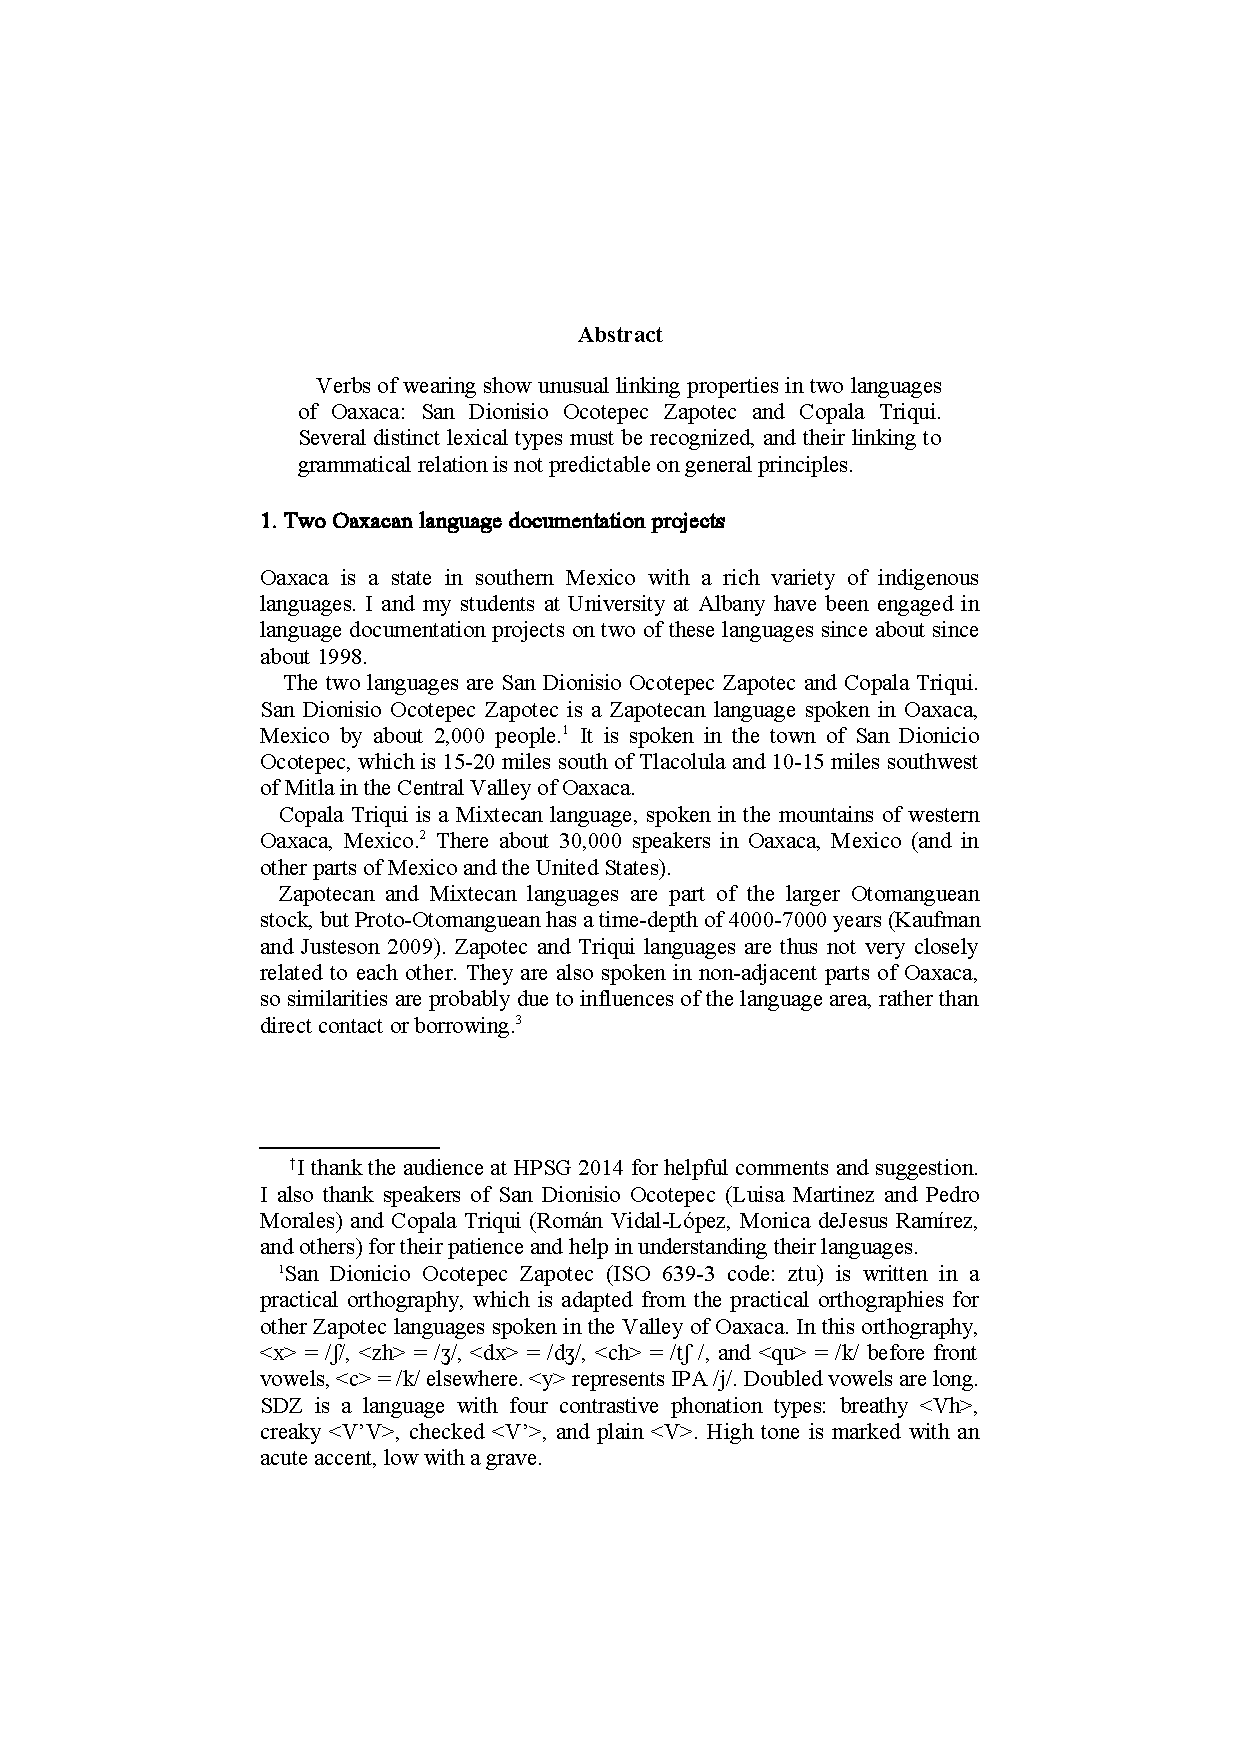
\includepdf[pages=-,pagecommand=\thispagestyle{plain}]{Includes/broadwell.pdf}
        \setcounter{page}{217}
        \phantomsection
        \addcontentsline{toc}{section}{Pegah Faghiri, Pollet Samvelian, Barbara Hemforth: Accessibility and Word Order: The Case of Ditransitive Constructions in Persian}
\thispagestyle{empty}

\begin{center}
  {\huge\bfseries Accessibility and Word Order: The Case of Ditransitive Constructions in Persian\par}

  \bigskip

~\\
\begingroup
\setlength{\leftskip}{0pt plus 1fill}
\setlength{\rightskip}{0pt plus 1fill}
\setlength{\parindent}{0pt}
\setlength{\parfillskip}{0pt}
  \formatauthor{Pegah Faghiri}{\begin{tabular}{@{}c@{}}Université Sorbonne Nouvelle\end{tabular}}
\formatauthor{Pollet Samvelian}{\begin{tabular}{@{}c@{}}Université Sorbonne Nouvelle\end{tabular}}
\formatauthor{Barbara Hemforth}{\begin{tabular}{@{}c@{}}CNRS/Laboratoire de Linguistique Formelle (LLF)\end{tabular}}

\par\endgroup

  \vspace*{8ex}

  Proceedings of the 21st International Conference on\par Head-Driven Phrase Structure Grammar

  \bigskip

  University at Buffalo

  \medskip

  Stefan Müller (Editor)

  \medskip

  2014

  \medskip

  CSLI Publications

  \medskip

  pages 217--237

  \medskip

  \url{http://csli-publications.stanford.edu/HPSG/2014}
\end{center}
\vfill

\noindent



\vfill
\noindent
% APA Style
Faghiri, Pegah, Samvelian, Pollet, \& Hemforth, Barbara. 2014. Accessibility and Word Order: The Case of Ditransitive Constructions in Persian. In Müller, Stefan (Ed.), \emph{{Proceedings of the 21st International Conference on Head-Driven Phrase Structure Grammar, University at Buffalo}}, 217--237. Stanford,
CA: CSLI Publications. \hfill\href{http://creativecommons.org/licenses/by/4.0/}{\includegraphics[height=.75em]{Includes/ccby.eps}}

\newpage
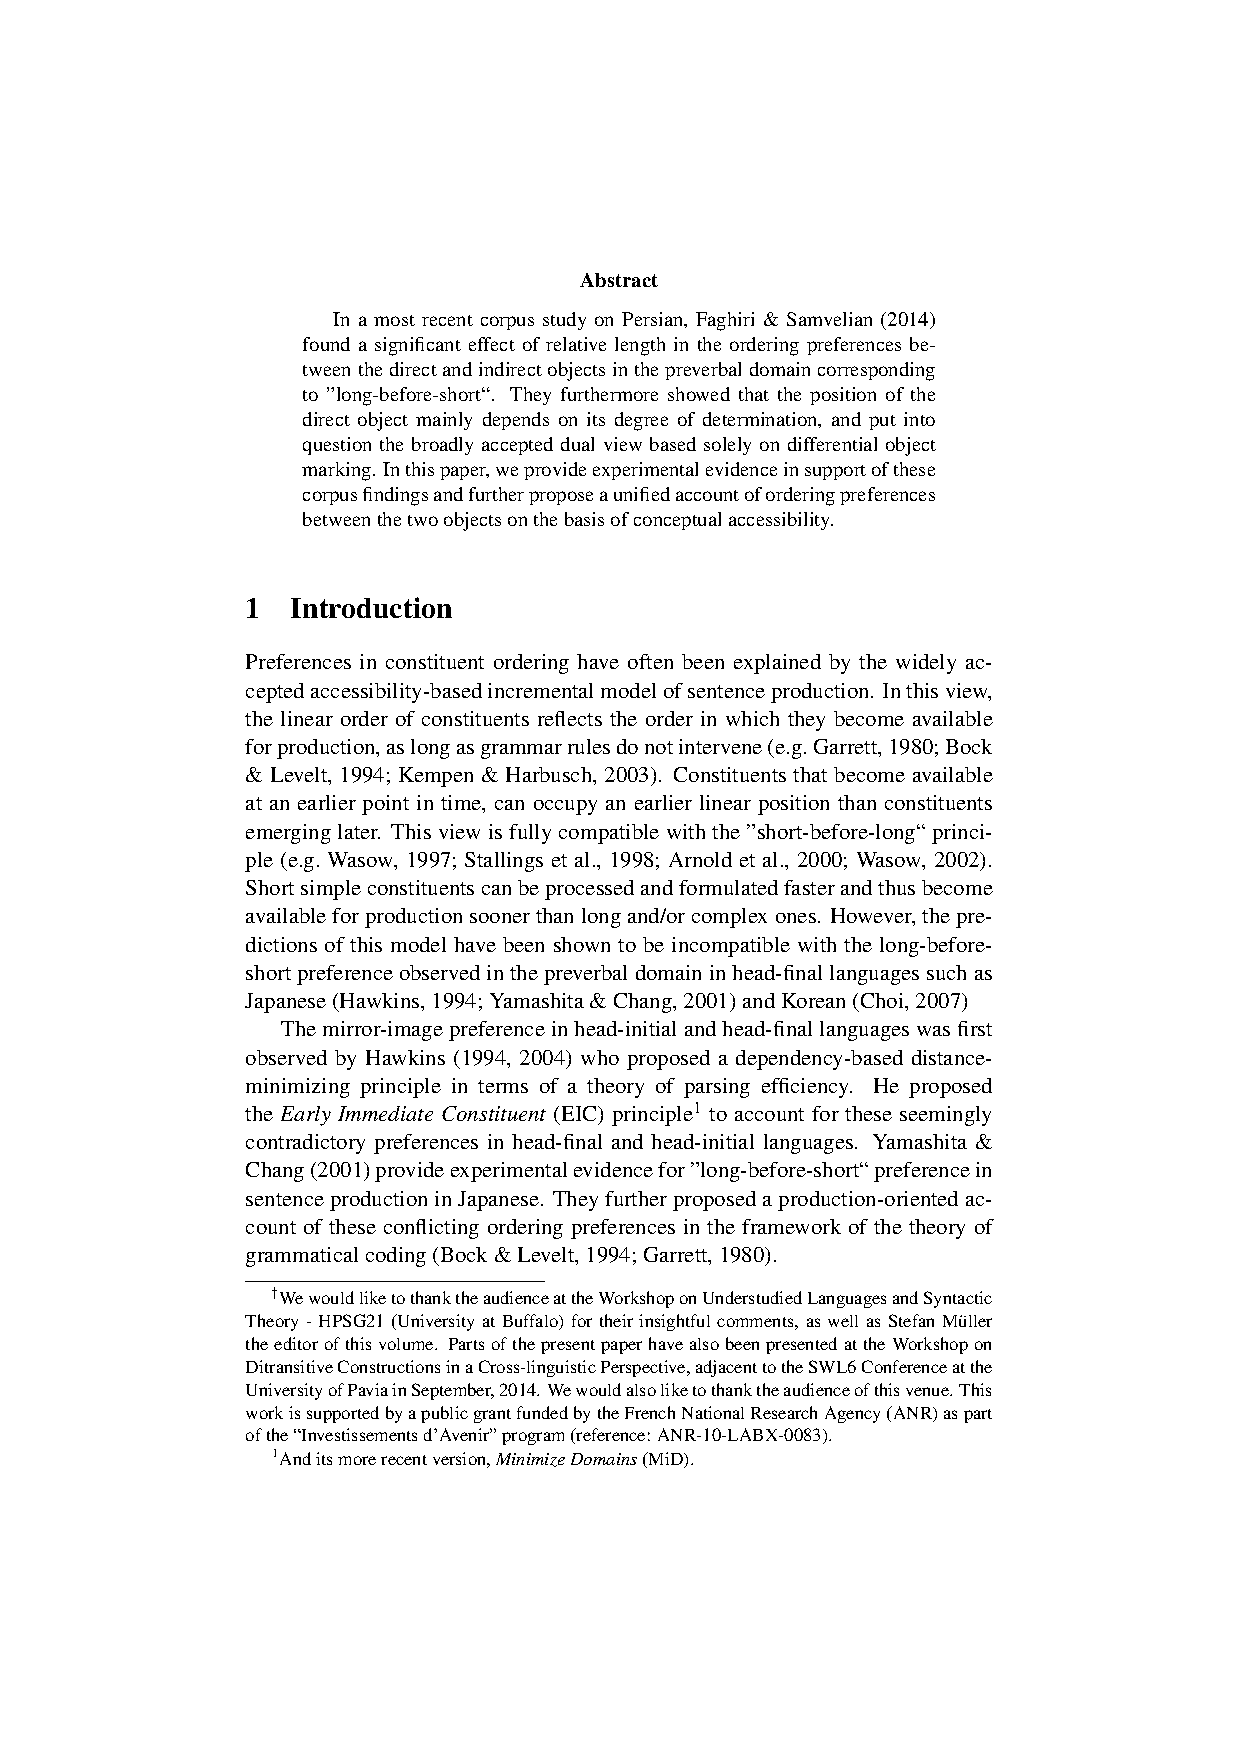
\includepdf[pages=-,pagecommand=\thispagestyle{plain}]{Includes/fsh.pdf}
        \setcounter{page}{238}
        \phantomsection
        \addcontentsline{toc}{section}{Michael Hahn: Predication and NP Structure in an Omnipredicative Language: The Case of Khoekhoe}
\thispagestyle{empty}

\begin{center}
  {\huge\bfseries Predication and NP Structure in an Omnipredicative Language: The Case of Khoekhoe\par}

  \bigskip

~\\
\begingroup
\setlength{\leftskip}{0pt plus 1fill}
\setlength{\rightskip}{0pt plus 1fill}
\setlength{\parindent}{0pt}
\setlength{\parfillskip}{0pt}
  \formatauthor{Michael Hahn}{\begin{tabular}{@{}c@{}}University of Tübingen\end{tabular}}

\par\endgroup

  \vspace*{8ex}

  Proceedings of the 21st International Conference on\par Head-Driven Phrase Structure Grammar

  \bigskip

  University at Buffalo

  \medskip

  Stefan Müller (Editor)

  \medskip

  2014

  \medskip

  CSLI Publications

  \medskip

  pages 238--258

  \medskip

  \url{http://csli-publications.stanford.edu/HPSG/2014}
\end{center}
\vfill

\noindent



\vfill
\noindent
% APA Style
Hahn, Michael. 2014. Predication and NP Structure in an Omnipredicative Language: The Case of Khoekhoe. In Müller, Stefan (Ed.), \emph{{Proceedings of the 21st International Conference on Head-Driven Phrase Structure Grammar, University at Buffalo}}, 238--258. Stanford,
CA: CSLI Publications. \hfill\href{http://creativecommons.org/licenses/by/4.0/}{\includegraphics[height=.75em]{Includes/ccby.eps}}

\newpage
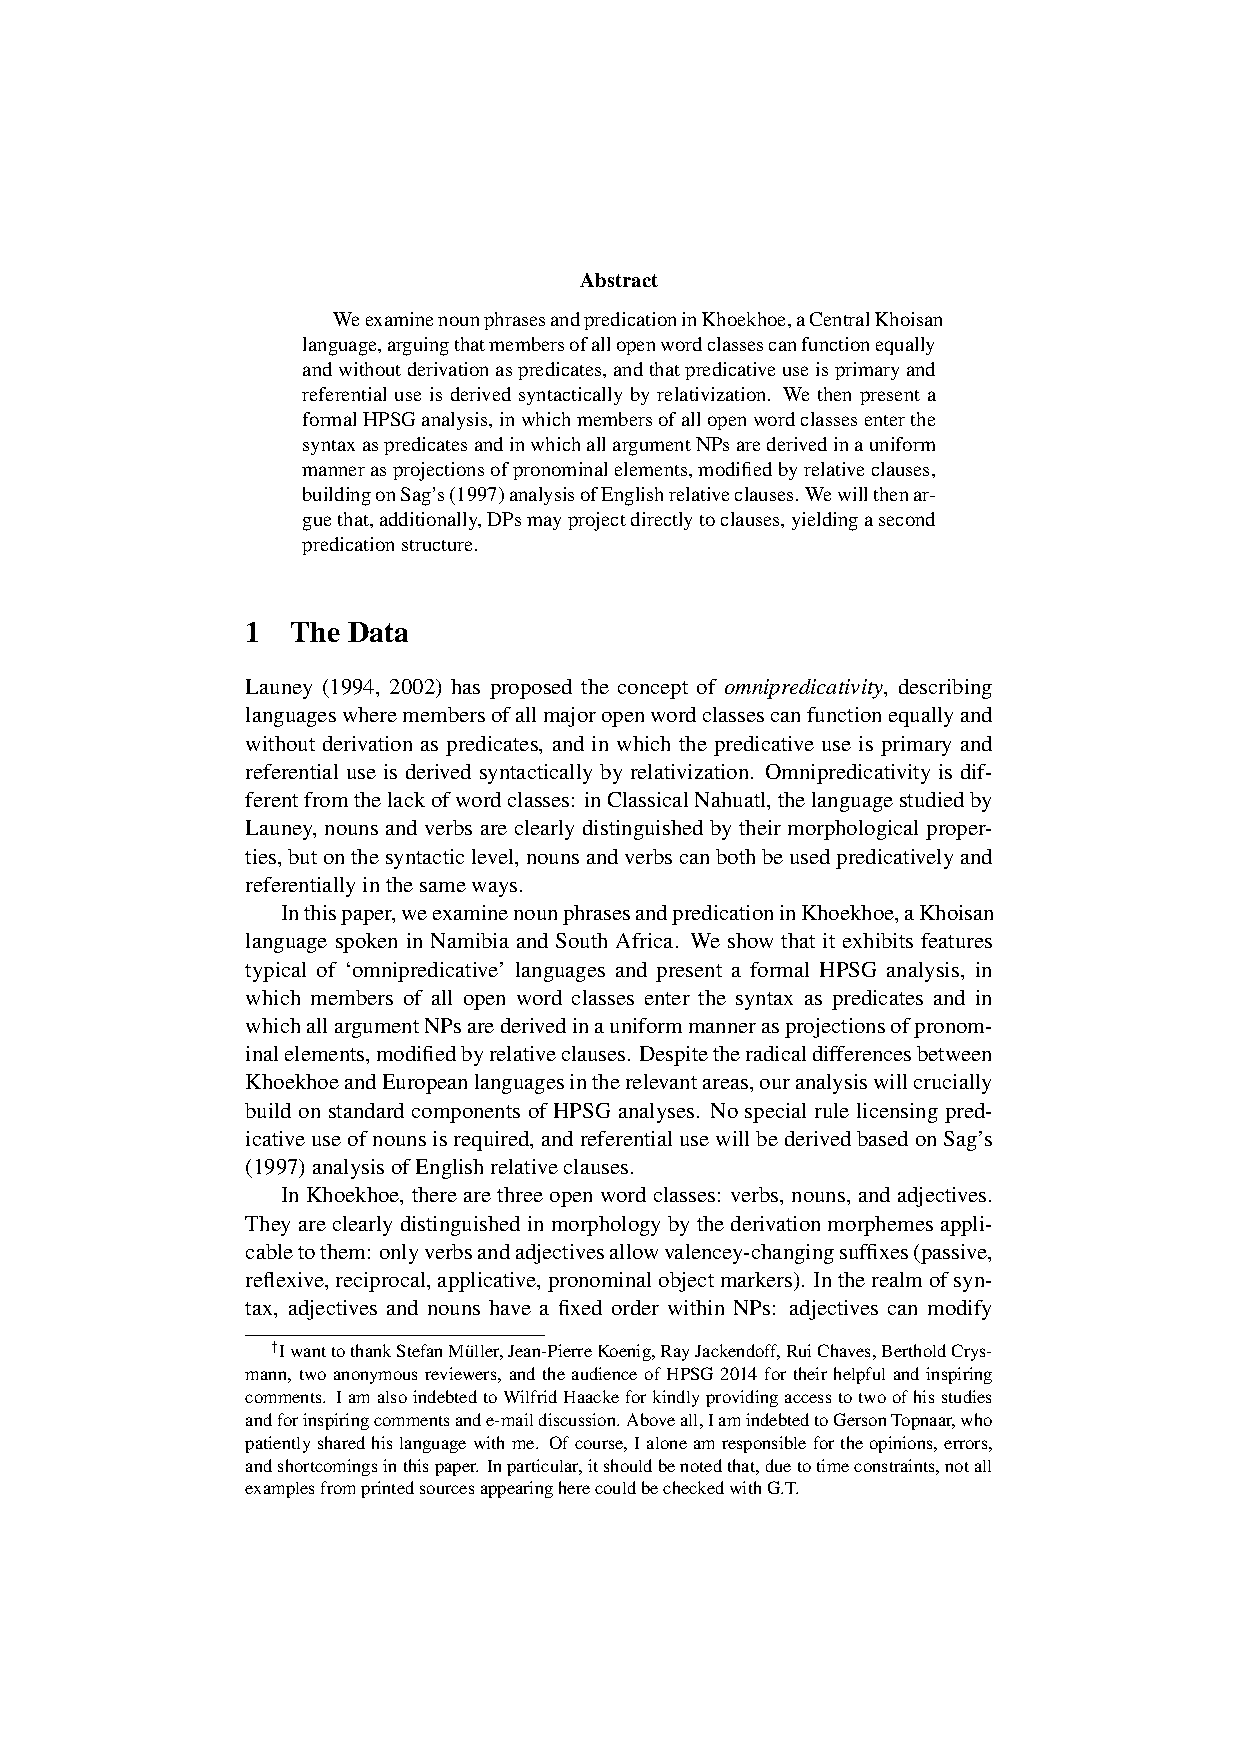
\includepdf[pages=-,pagecommand=\thispagestyle{plain}]{Includes/hahn.pdf}
        \setcounter{page}{259}
        \phantomsection
        \addcontentsline{toc}{section}{Shrita Hassamal, Anne. Abeill{\'e}: Degree adverbs in Mauritian}
\thispagestyle{empty}

\begin{center}
  {\huge\bfseries Degree adverbs in Mauritian\par}

  \bigskip

~\\
\begingroup
\setlength{\leftskip}{0pt plus 1fill}
\setlength{\rightskip}{0pt plus 1fill}
\setlength{\parindent}{0pt}
\setlength{\parfillskip}{0pt}
  \formatauthor{Shrita Hassamal}{\begin{tabular}{@{}c@{}}LLF, CNRS, Université Paris Diderot\end{tabular}}
\formatauthor{Anne. Abeillé}{\begin{tabular}{@{}c@{}}IUF, LLF, CNRS, Université Paris Diderot\end{tabular}}

\par\endgroup

  \vspace*{8ex}

  Proceedings of the 21st International Conference on\par Head-Driven Phrase Structure Grammar

  \bigskip

  University at Buffalo

  \medskip

  Stefan Müller (Editor)

  \medskip

  2014

  \medskip

  CSLI Publications

  \medskip

  pages 259--279

  \medskip

  \url{http://csli-publications.stanford.edu/HPSG/2014}
\end{center}
\vfill

\noindent



\vfill
\noindent
% APA Style
Hassamal, Shrita, \& Abeillé, Anne. 2014. Degree adverbs in Mauritian. In Müller, Stefan (Ed.), \emph{{Proceedings of the 21st International Conference on Head-Driven Phrase Structure Grammar, University at Buffalo}}, 259--279. Stanford,
CA: CSLI Publications. \hfill\href{http://creativecommons.org/licenses/by/4.0/}{\includegraphics[height=.75em]{Includes/ccby.eps}}

\newpage
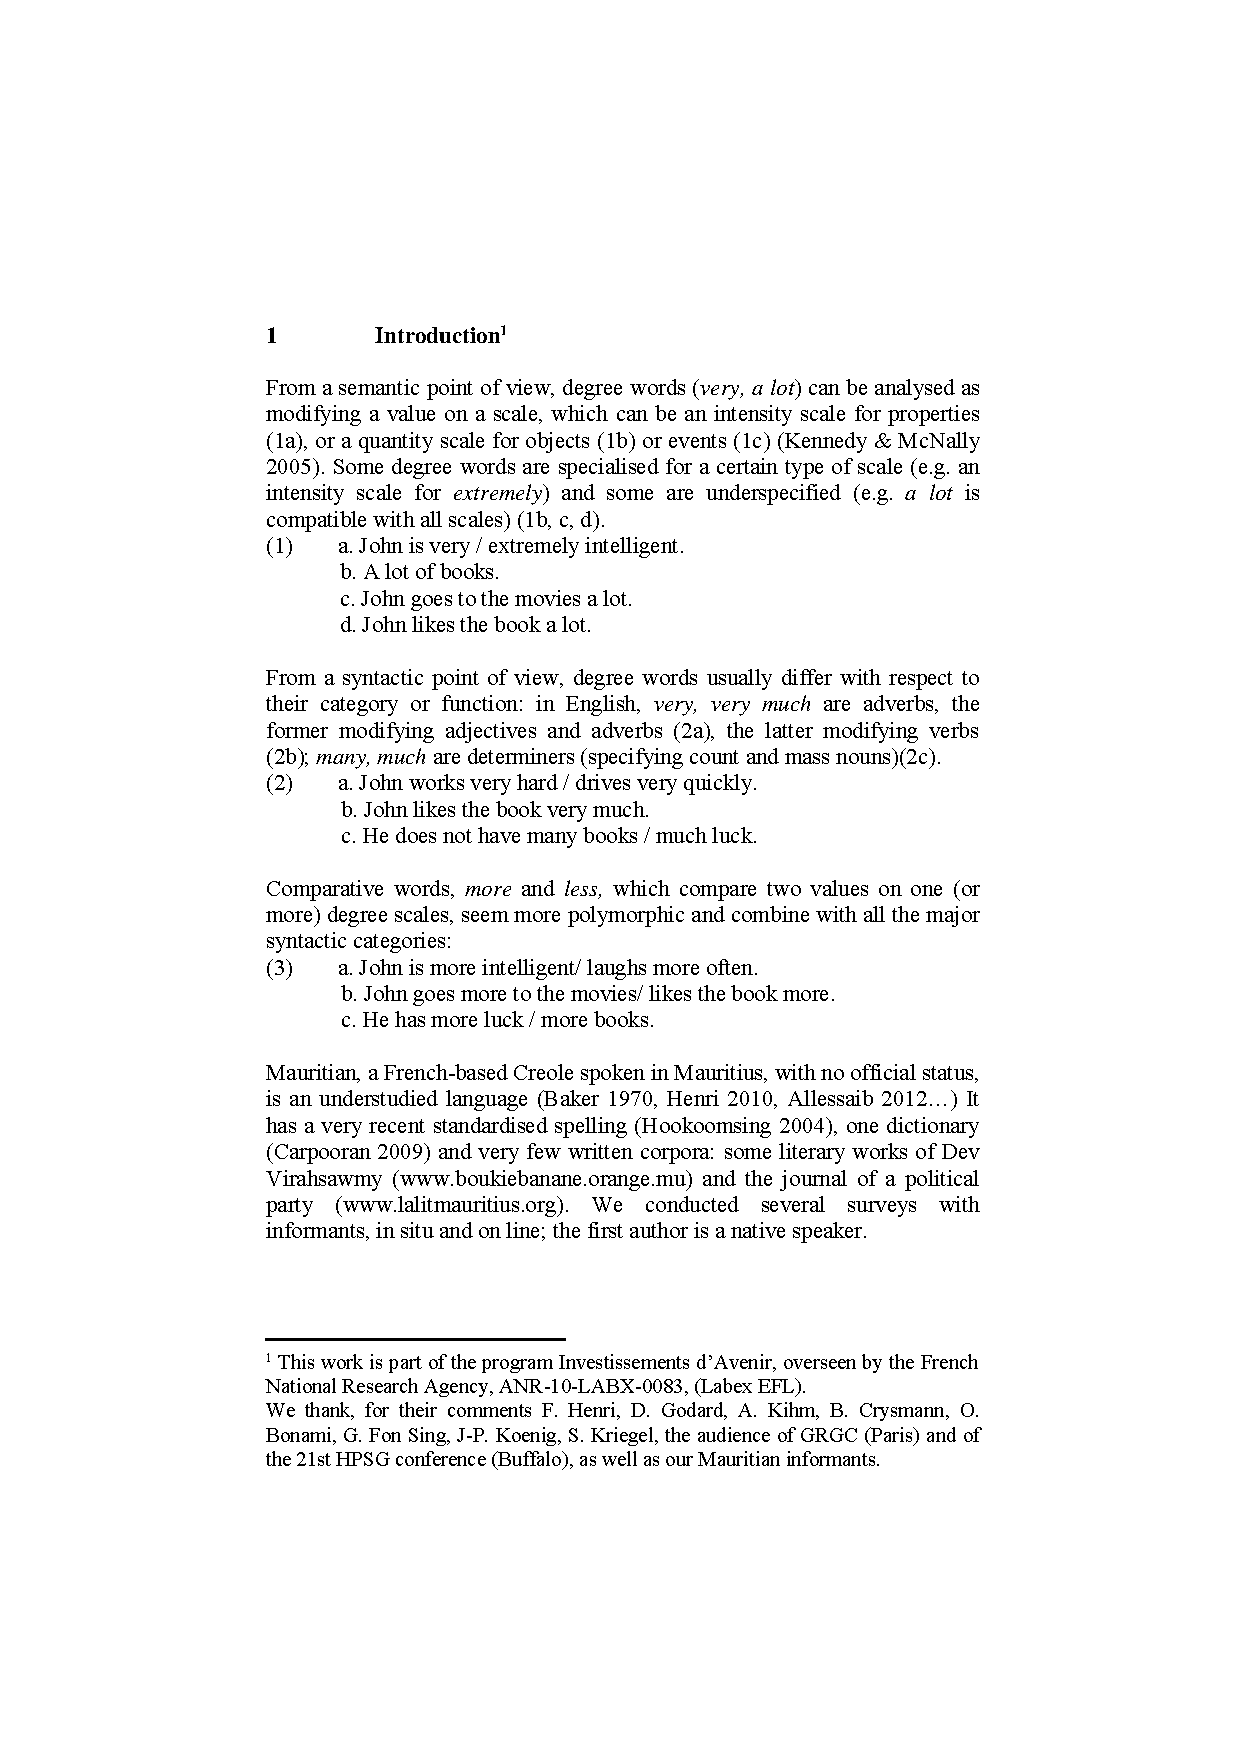
\includepdf[pages=-,pagecommand=\thispagestyle{plain}]{Includes/hassamal-abeille.pdf}
        \setcounter{page}{280}
        \phantomsection
        \addcontentsline{toc}{section}{Dong-yi Lin: Obligatory Control and Event Structure in Kavalan}
\thispagestyle{empty}

\begin{center}
  {\huge\bfseries Obligatory Control and Event Structure in Kavalan\par}

  \bigskip

~\\
\begingroup
\setlength{\leftskip}{0pt plus 1fill}
\setlength{\rightskip}{0pt plus 1fill}
\setlength{\parindent}{0pt}
\setlength{\parfillskip}{0pt}
  \formatauthor{Dong-yi Lin}{\begin{tabular}{@{}c@{}}Ghent University\end{tabular}}

\par\endgroup

  \vspace*{8ex}

  Proceedings of the 21st International Conference on\par Head-Driven Phrase Structure Grammar

  \bigskip

  University at Buffalo

  \medskip

  Stefan Müller (Editor)

  \medskip

  2014

  \medskip

  CSLI Publications

  \medskip

  pages 280--298

  \medskip

  \url{http://csli-publications.stanford.edu/HPSG/2014}
\end{center}
\vfill

\noindent



\vfill
\noindent
% APA Style
Lin, Dong-yi. 2014. Obligatory Control and Event Structure in Kavalan. In Müller, Stefan (Ed.), \emph{{Proceedings of the 21st International Conference on Head-Driven Phrase Structure Grammar, University at Buffalo}}, 280--298. Stanford,
CA: CSLI Publications. \hfill\href{http://creativecommons.org/licenses/by/4.0/}{\includegraphics[height=.75em]{Includes/ccby.eps}}

\newpage
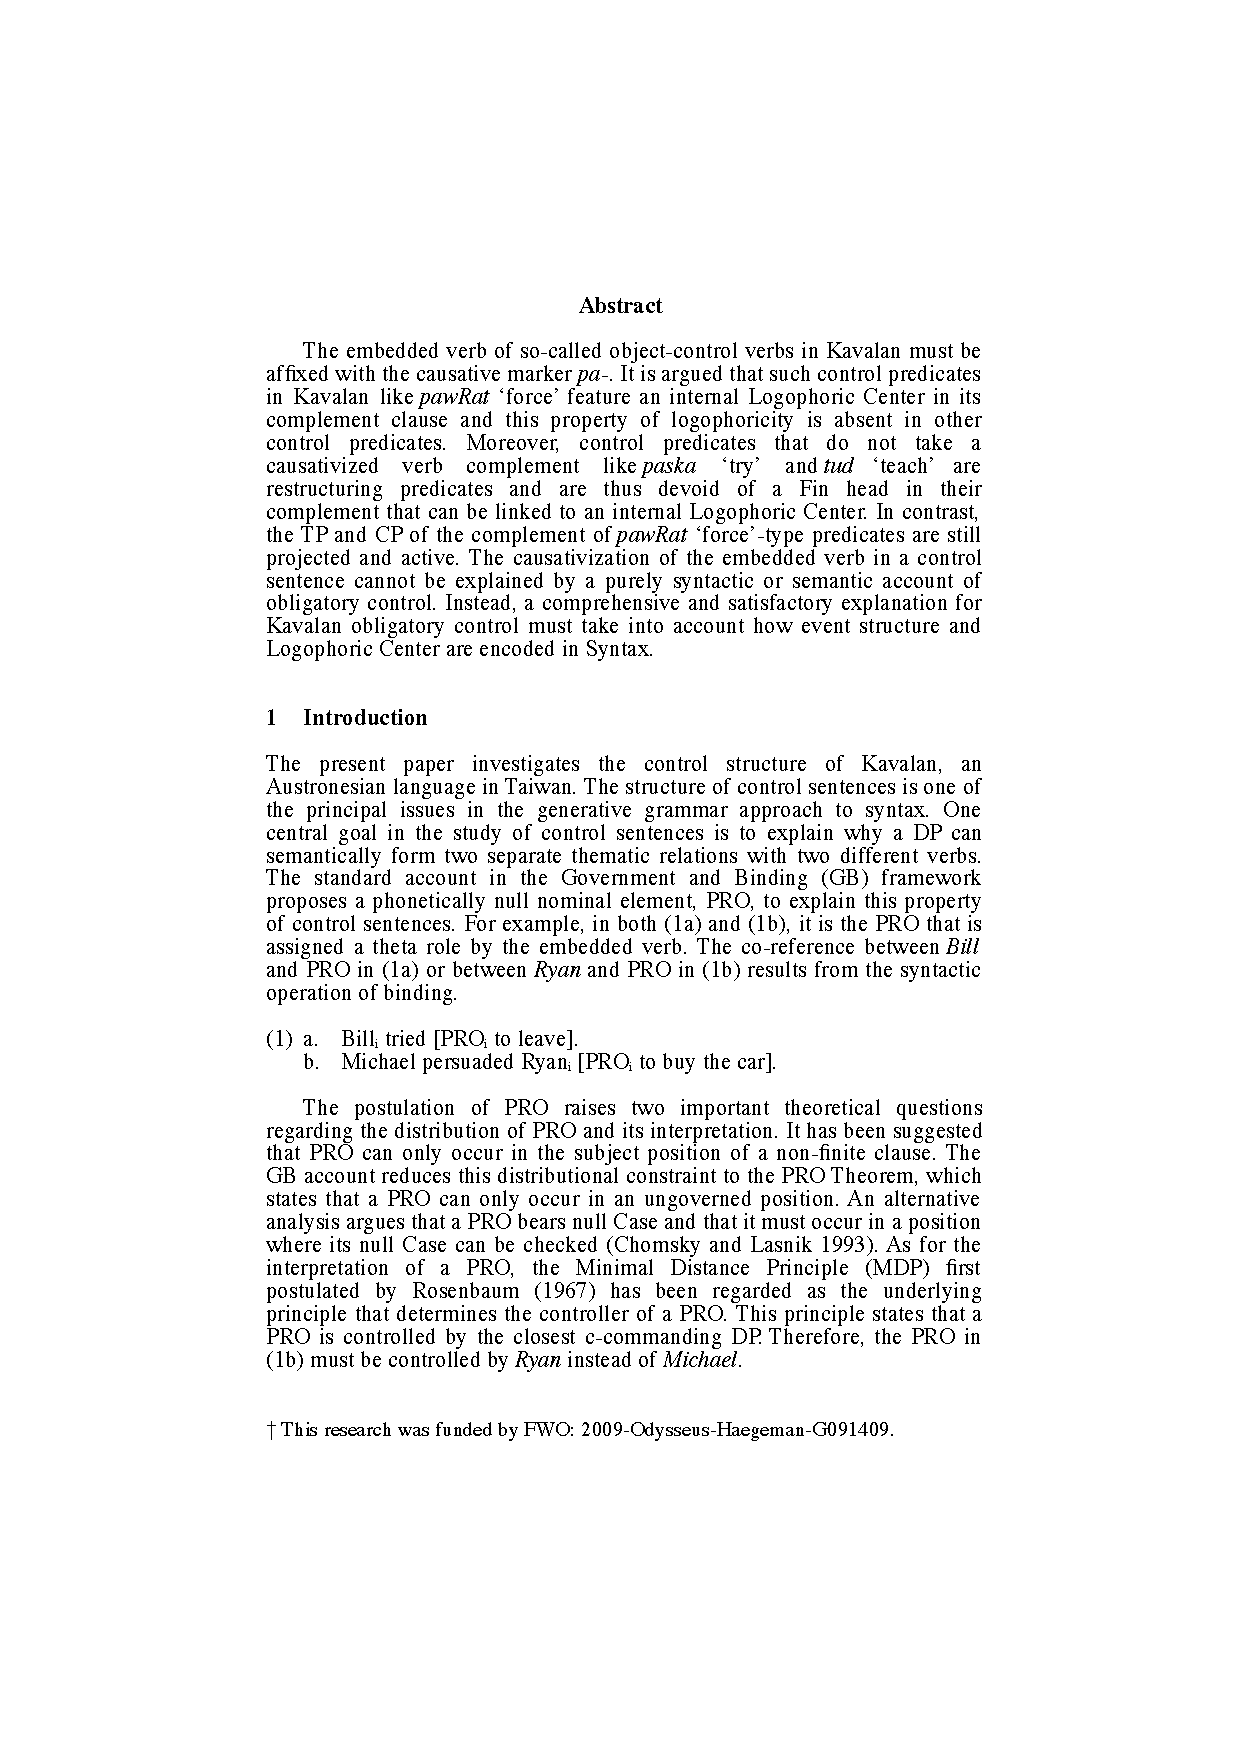
\includepdf[pages=-,pagecommand=\thispagestyle{plain}]{Includes/lin.pdf}
        \setcounter{page}{299}
        \phantomsection
        \addcontentsline{toc}{section}{Dejan Mati{\'c}, Irina Nikolaeva: Focus feature
percolation: Evidence from Tundra Nenets and Tundra Yukaghir}
\thispagestyle{empty}

\begin{center}
  {\huge\bfseries Focus feature
percolation: Evidence from Tundra Nenets and Tundra Yukaghir\par}

  \bigskip

~\\
\begingroup
\setlength{\leftskip}{0pt plus 1fill}
\setlength{\rightskip}{0pt plus 1fill}
\setlength{\parindent}{0pt}
\setlength{\parfillskip}{0pt}
  \formatauthor{Dejan Matić}{\begin{tabular}{@{}c@{}}Max Planck Institute for Psycholinguistics, Nijmegen\end{tabular}}
\formatauthor{Irina Nikolaeva}{\begin{tabular}{@{}c@{}}SOAS, University of London\end{tabular}}

\par\endgroup

  \vspace*{8ex}

  Proceedings of the 21st International Conference on\par Head-Driven Phrase Structure Grammar

  \bigskip

  University at Buffalo

  \medskip

  Stefan Müller (Editor)

  \medskip

  2014

  \medskip

  CSLI Publications

  \medskip

  pages 299--317

  \medskip

  \url{http://csli-publications.stanford.edu/HPSG/2014}
\end{center}
\vfill

\noindent



\vfill
\noindent
% APA Style
Matić, Dejan, \& Nikolaeva, Irina. 2014. Focus feature
percolation: Evidence from Tundra Nenets and Tundra Yukaghir. In Müller, Stefan (Ed.), \emph{{Proceedings of the 21st International Conference on Head-Driven Phrase Structure Grammar, University at Buffalo}}, 299--317. Stanford,
CA: CSLI Publications. \hfill\href{http://creativecommons.org/licenses/by/4.0/}{\includegraphics[height=.75em]{Includes/ccby.eps}}

\newpage
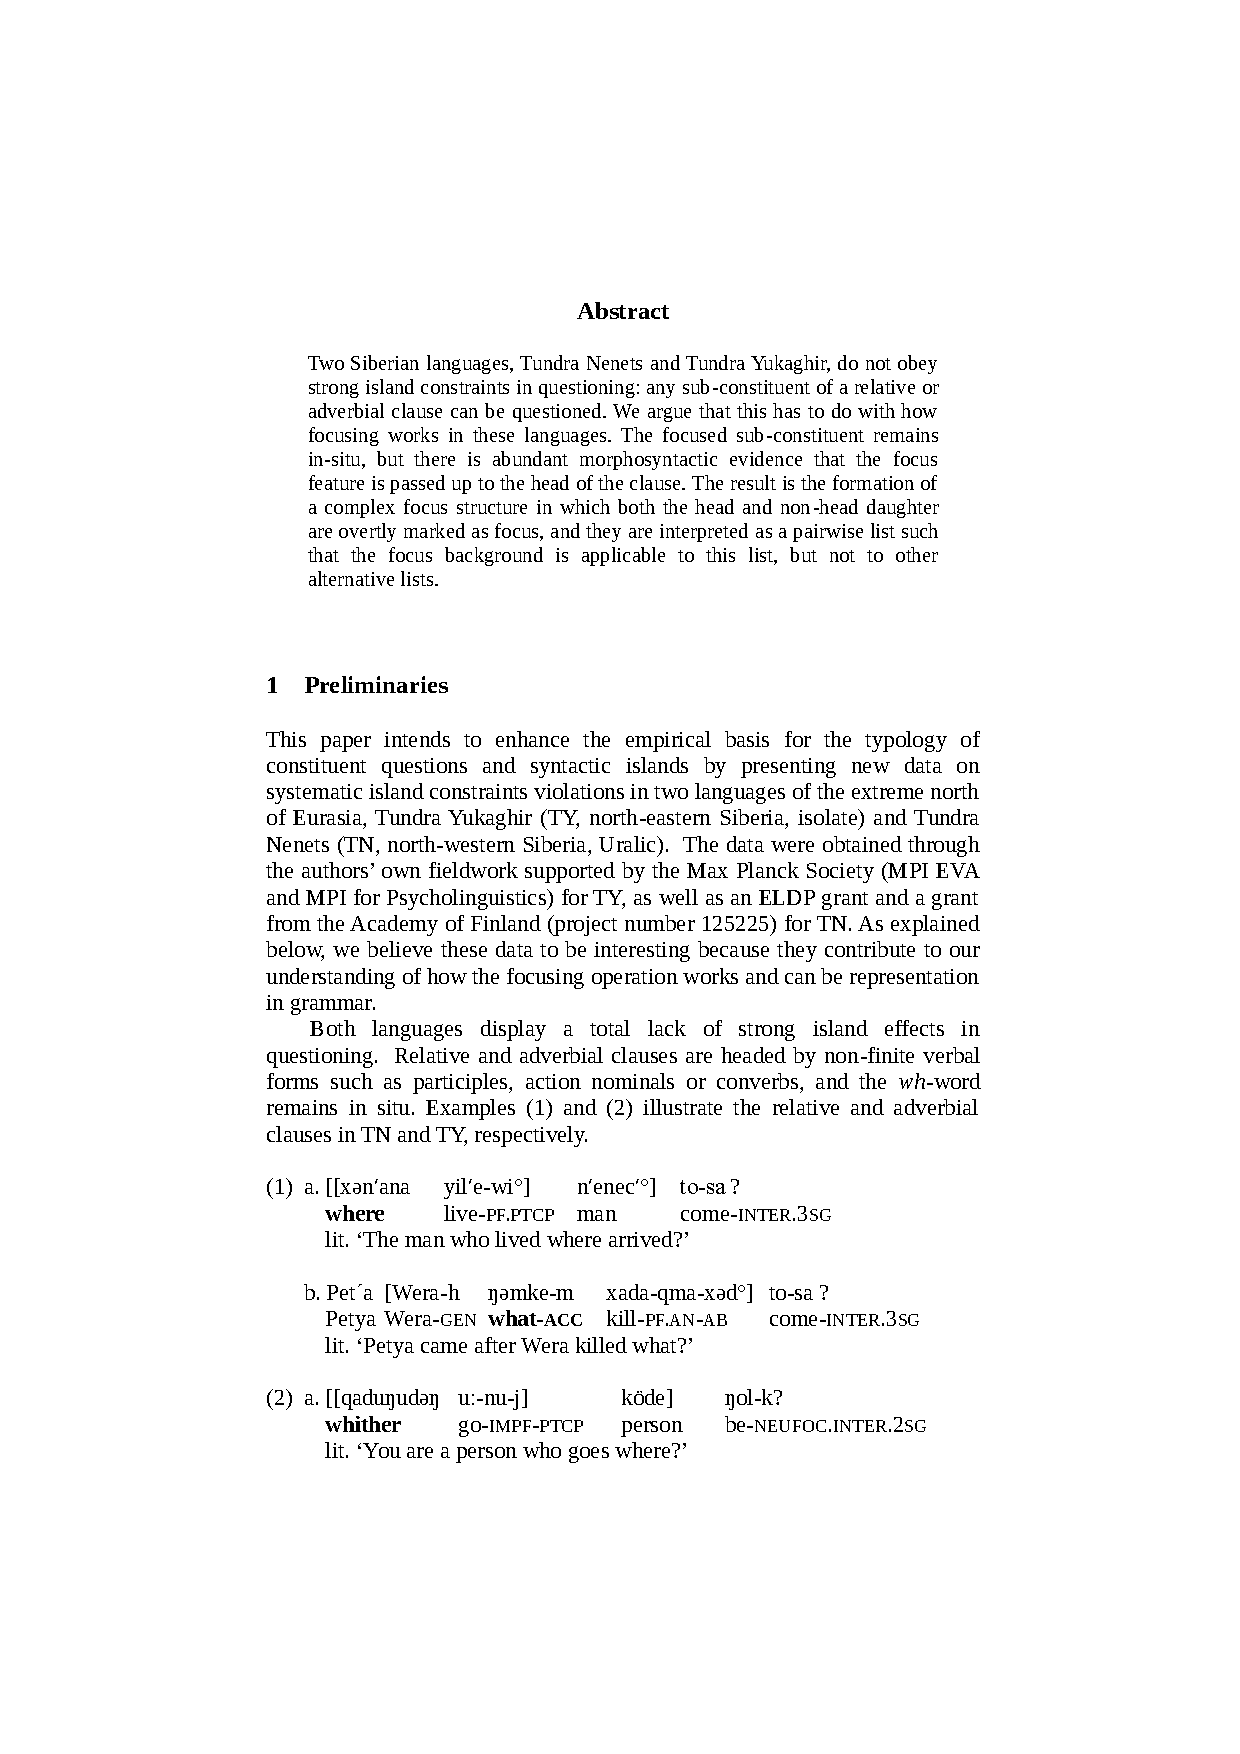
\includepdf[pages=-,pagecommand=\thispagestyle{plain}]{Includes/matic-nikolaeva.pdf}
\end{document}
